\documentclass[12pt, titlepage]{article}
%\documentclass[12pt, titlepage, draft]{article}
\usepackage[affil-it]{authblk}

\usepackage{geometry}                % See geometry.pdf to learn the layout options. There are lots.
\geometry{letterpaper}                   % ... or a4paper or a5paper or ... 
\setcounter{secnumdepth}{3}
\setcounter{tocdepth}{3}

\usepackage{graphicx}
\usepackage{epstopdf}

\usepackage{amsmath}
\usepackage{amssymb}
\usepackage{amsfonts}
\usepackage{mathrsfs, bm}
\usepackage{booktabs}
\usepackage{verbatim}
\usepackage{natbib}
\usepackage{setspace}
%\doublespace
\onehalfspace
\usepackage{lscape}
\usepackage{multirow}
\usepackage{grffile}
\usepackage{lineno}
\usepackage{enumerate}
\usepackage{multicol}

\usepackage[hyphens]{url}
\usepackage{hyperref}

\usepackage[labelfont=bf]{caption}

\usepackage{ifpdf}
\ifpdf
	\DeclareGraphicsRule{.tif}{png}{.png}{`convert #1 `dirname #1`/`basename #1 .tif`.png}
	\DeclareGraphicsRule{*}{mps}{*}{}
\fi

\usepackage{xcolor}
\definecolor{dark-red}{rgb}{0.4,0.15,0.15}
\definecolor{dark-blue}{rgb}{0.15,0.15,0.4}
\definecolor{medium-blue}{rgb}{0,0,0.5}
\hypersetup{
    colorlinks, linkcolor={dark-red},
    citecolor={dark-blue}, urlcolor={medium-blue}
}

\geometry{letterpaper,tmargin=1in,bmargin=1in,lmargin=1in,rmargin=1in}

\setlength{\parindent}{0.0in}
\setlength{\parskip}{0.1in}



%\numberwithin{equation}{section}
%\numberwithin{figure}{section}

%%%%%%%%%%%%%%%%%%%%%%%%%%%%%% Textclass specific LaTeX commands.

\newenvironment{lyxcode}
{\begin{list}{}{
\setlength{\rightmargin}{\leftmargin}
\setlength{\listparindent}{0pt}% needed for AMS classes
\raggedright
\setlength{\itemsep}{0pt}
\setlength{\parsep}{0pt}
\normalfont\ttfamily}%
 \item[]}
{\end{list}}



\usepackage[margins]{../../trackchanges-0.7.0/LatexPackage/trackchanges}

%%%%%%%%%%%%%%%%%%%%%%%%%%%%%%%%%%%%%%%%%%%%%%%%%%%%%%%%

%\title{ AIMBAT: Automated and Interactive Measurement of Body wave Arrival Times \\ User Manual \\ Version 0.1.1}
\title{AIMBAT \\ User Manual \\ Version 0.1.1}

\author[1*]{Xiaoting Lou}
%\author[1]{Suzan van der Lee}
%\author[1,2]{Simon Lloyd}

\affil[1]{Department of Earth and Planetary Sciences, Northwestern University, Evanston, Illinois, USA}
%\affil[2]{Now at Department of Meteorology and Geophysics, University of Vienna, Austria}
\affil[*]{Email: xlou@u.northwestern.edu}

%\date{}


%%%%%%%%%%%%%%%%%%%%%%%%%%%%%%%%%%%%%%%%%%%%%%%%%%%%%%%%
\begin{document}
\maketitle

%\linenumbers
\tableofcontents


\newpage
%%%%%%%%%%%%%%%%%%%%%%%%%%%%%%%%%%%%%%%%%%%%%%%%%%%%%%%%
\section{Introduction}

AIMBAT (Automated and Interactive Measurement of Body wave Arrival Times) is an open-source software package for efficiently measuring teleseismic body wave arrival times for large seismic arrays \citep{pytool}.
It is based on a widely used method called MCCC (Multi-Channel Cross-Correlation) developed by \cite{mccc}.
The package is automated in the sense of initially aligning seismograms for MCCC which is achieved by an ICCS (Iterative Cross Correlation and Stack) algorithm.
Meanwhile, a GUI (graphical user interface) is built to perform seismogram quality control interactively.
Therefore, user processing time is reduced while valuable input from a user's expertise is retained. 
As a byproduct, SAC \citep{sac} plotting and phase picking functionalities are replicated and enhanced.

Modules and scripts included in the AIMBAT package were developed using Python programming language (\url{http://www.python.org}) and its open-source modules on the Mac OS X platform since 2009. The original MCCC code \citep{mccc} was transcribed into Python.
The GUI of AIMBAT was inspired and initiated at the 2009 EarthScope USArray Data Processing and Analysis Short Course (\url{http://www.iris.edu/hq/es\_course/}).
AIMBAT runs on Mac OS X, Linux/Unix and Windows thanks to the platform-independent feature of Python. 
It's been tested on Mac OS 10.6.8 and 10.7 and Fedora 16.

The AIMBAT software package is distributed under the GNU General Public License Version 3 (GPLv3) as published by the Free Software Foundation (\url{http://www.gnu.org/licenses/gpl.html}).




%%%%%%%%%%%%%%%%%%%%%%%%%%%%%%%%%%%%%%%%%%%%%%%%%%%%%%%%
\newpage
\section{Installation}


\subsection{Install Dependencies}

The AIMBAT package depends on the standard libraries of Python 2.7 (\url{http://docs.python.org/library/}), including 
\texttt{os}, 
\texttt{sys}, 
\texttt{ConfigParser(argparse)}, 
\texttt{optparse}, 
\texttt{contextlib}, 
\texttt{pickle/cPickle}, 
\texttt{gzip}, 
and
\texttt{bz2}.
%
AIMBAT also utilizes Numpy (\url{http://numpy.scipy.org}) and Scipy (\url{http://scipy.org}) for numerical array computation, and Matplotlib \citep{matplotlib} for 2-D plotting and GUI applications.
These packages need to be installed before using AIMBAT.

\subsubsection{Mac}

For Mac users, we recommend Macports (\url{http://http://www.macports.org/}) to install the dependent packages of AIMBAT. 
After installing Macports, run the following commands with superuser privilege:

\begin{lyxcode}
port install python27

port install py27-numpy

port install py27-scipy

port install py27-matplotlib

port install py27-ipython

port install python\_select

\end{lyxcode}

Python 2.7 is thus installed to the \url{<prefix>} directory, which is
\url{/opt/local/Library/Frameworks/Python.framework/Versions/2.7} for this case.
Corresponding packages Numpy, Scipy and Matplotlib are installed to the global site-packages directory
\url{<prefix>/lib/python2.7/site-packages}.

Installation of the last two packages are optional. 
\texttt{ipython} is an enhanced interactive Python shell.
\texttt{python\_select} is used to select default Python version by the following command:

\begin{lyxcode}
port select --set python python27
\end{lyxcode}


\subsubsection{Linux}

For Linux users, package management tools work similarly, such as \texttt{yum} on Red Hat/Fedora system:

\begin{lyxcode}

yum install python.x86\_64

yum install numpy.x86\_64

yum install scipy.x86\_64

yum install python-matplotlib.x86\_64

\end{lyxcode}

and \texttt{aptitude} on Debian system: 

\begin{lyxcode}
aptitude install python

aptitude install python-numpy

aptitude install python-scipy 

aptitude install python-matplotlib

\end{lyxcode}


The \url{<prefix>} directory is \url{/usr}.

%%%%%%%%%%%%%%%%%%%%%%%%%%%%
\subsection{Install pysmo.sac and pysmo.aimbat}

AIMBAT is released as a sub-package of pysmo in the name of \texttt{pysmo.aimbat} along with another sub-package \texttt{pysmo.sac}.
The latest releases of \texttt{pysmo.sac} and \texttt{pysmo.aimbat} are available for download at both

\begin{lyxcode}
\url{http://www.earth.northwestern.edu/~xlou/aimbat.html}
\end{lyxcode}

and github:

\begin{lyxcode}
https://github.com/pysmo/sac

https://github.com/pysmo/aimbat
\end{lyxcode}


Decompress the gzipped source tar balls in the directory where you want to install the packages (\url{<pkg-install-dir>}):

\begin{lyxcode}
tar zxvf pysmo-sac-0.5.tar.gz

tar zxvf pysmo-aimbat-0.1.1.tar.gz
\end{lyxcode}





%%%%%%%%%%%%%%%%
\subsubsection{Install pysmo.sac}

Python module \texttt{Distutils} is used to write a \texttt{setup.py} script to easily build, distribute, and install \texttt{pysmo.sac}.
In the directory \url{<pkg-install-dir>/pysmo-sac-0.5}, type

\begin{lyxcode}
python setup.py build

python setup.py install
\end{lyxcode}

to install it and its package information file \texttt{pysmo.sac-0.5-py2.7.egg-info} to the global site-packages directory \url{<prefix>/lib/python2.7/site-packages}, which is the same as Numpy, Scipy, and Matplotlib.

If you don't have write permission to the global site-packages directory, use the "\texttt{--user}" option to install to
\url{<userbase>/lib/python2.7/site-packages}:

\begin{lyxcode}
python setup.py install --user
\end{lyxcode}


%%%%%%%%%%%%%%%%
\subsubsection{Install pysmo.aimbat}

Three sub-directories are included in the \url{<pkg-install-dir>/pysmo-aimbat-0.1.1} directory: \texttt{example}, \texttt{scripts} and \texttt{src}, which contain example SAC data files, Python scripts to run at command line, and Python modules to install, respectively.


The core cross-correlation functions in \texttt{pysmo.aimbat} are written in both Python/Numpy (\texttt{xcorr.py}) and Fortran (\texttt{xcorr.f90}). 
Therefore, we need to use Numpy's \texttt{Distutils} module for enhanced support of Fortran extension. 
The usage is similar to the standard \texttt{Distutils}.

In the directory \url{<pkg-install-dir>/pysmo-aimbat-0.1.1}, type

\begin{lyxcode}
python setup.py build --fcompiler=gfortran

python setup.py install
\end{lyxcode}

to install the \texttt{src} directory to \url{<prefix>/lib/python2.7/site-packages/pysmo/aimbat}.
Other Fortran compilers can be specified instead of gfortran.


Add \url{<pkg-install-dir>/pysmo-aimbat-0.1.1/scripts} to environment variable \texttt{PATH} in a shell's start-up file for command line execution of the scripts. Typically for Bash and C shell users, type 

\begin{lyxcode}
export PATH=\$PATH:<pkg-install-dir>/pysmo-aimbat-0.1.1/scripts

setenv PATH \$PATH:<pkg-install-dir>/pysmo-aimbat-0.1.1/scripts
\end{lyxcode}

in \texttt{.bashrc} and \texttt{.cshrc} files, respectively.

To test the installation of the \texttt{pysmo.sac} and \texttt{pysmo.aimbat} packages, type

\begin{lyxcode}
from pysmo import sac

from pysmo import aimbat

\end{lyxcode}

in a Python shell.



\newpage
%%%%%%%%%%%%%%%%%%%%%%%%%%%%%%%%%%%%%%%%%%%%%%%%%%%%%%%%
\section{Tutorial}

%%%%%%%%%%%%%%%%%%%%%%%%%%%%
\subsection{Parameter Configuration}



Matplotlib works with six GUI (Graphical User Interface) toolkits: WX, Tk, Qt(4), GTK, Fltk and macosx (\url{http://matplotlib.org/contents.html}).
The GUI of AIMBAT utilizes GUI neutral widgets and GUI neutral event handling API (Application Programming Interface) to support interactive plotting (\url{http://matplotlib.org/api/widgets_api.html}, \url{http://matplotlib.org/users/event_handling.html}). 
Examples given in this manual are using the default toolkit \texttt{Tk} and backend \texttt{TkAgg}.
See \url{http://matplotlib.org/faq/usage_faq.html#what-is-a-backend}
and
\url{http://matplotlib.org/users/customizing.html#customizing-matplotlib}
for explanation of the backend and how to customize it. 
In short, put the following line in your \texttt{matplotlibrc} file:

\begin{lyxcode}
backend : TkAgg  \#Agg rendering to a Tk canvas 
\end{lyxcode}


Other parameters for the package can be set up by a configuration file \texttt{ttdefaults.conf}, which is interpreted by the module \texttt{ConfigParser}. 
This configuration file is searched in the following order:
\begin{enumerate}[(1)]
	\item file \texttt{ttdefaults.conf} in the current working directory
	\item file \texttt{.aimbat/ttdefaults.conf} in your \texttt{HOME} directory
	\item a file specified by environment variable \texttt{TTCONFIG} 
	\item file \texttt{ttdefaults.conf} in the directory where AIMBAT is installed 
\end{enumerate}

An example of the \texttt{ttdefaults.conf} file and its explanations are given in Table \ref{table:config}.

Python scripts in the \texttt{<pkg-install-dir>/pysmo-aimbat-0.1.1/scripts} can be executed from the command line. 
The command line arguments are parsed by the \texttt{optparse} module to improve the scripts' flexibility. 
If conflicts existed, the command line options override the default parameters given in the configuration file \texttt{ttdefaults.conf}.
Run the scripts with the "-h" option for the usage messages.


\begin{table}[h!]
\centering
{\scriptsize
\begin{tabular}{l l}
\toprule
File \texttt{ttdefaults.conf} 	& Description \\
\midrule
%%%%%%%%%%%%%%
$[$sacplot$]$ 			& \\
colorwave = blue		& Color of waveform \\
colorwavedel = gray		& Color of waveform which is deselected \\
colortwfill = green		& Color of time window fill \\
colortwsele = red		& Color of time window selection \\
alphatwfill = 0.2			& Transparency of time window fill \\
alphatwsele = 0.6		& Transparency of time window selection \\
npick = 6				& Number of time picks (plot picks: t0-t5) \\
pickcolors = kmrcgyb	& Colors of time picks \\
pickstyles = -- :			& Line styles of time picks (use second one if ran out of color)\\
figsize = 8 10			& Figure size for \texttt{plotphase.py} \\
rectseis = 0.1 0.06 0.76 0.9 & Axes rectangle size within the figure \\
minspan = 5 			& Minimum sample points for SpanSelector to select time window \\
srate = -1 				& Sample rate for loading SAC data. Read from first file if srate $<$ 0 \\

%%%%%%%%%%%%%%
\cmidrule(l){1-1}
$[$sachdrs$]$			& \\
twhdrs = user8 	user9	& SAC headers for time window beginning and ending \\
ichdrs = t0 t1 t2			& SAC headers for ICCS time picks \\
mchdrs = t2 t3			& SAC headers for MCCC input and output time picks \\
hdrsel = kuser0			& SAC header for seismogram selection status \\
qfactors = ccc snr coh	& Quality factors: cross-correlation coefficient, signal-to-noise ratio, time domain coherence \\
qheaders = user0 user1 user2		& SAC Headers for quality factors \\
qweights = 0.3333 0.3333 0.3333	& Weights for quality factors \\
%%%%%%%%%%%%%%
\cmidrule(l){1-1}
$[$iccs$]$				& \\
srate = -1 				& Sample rate for loading SAC data. Read from first file if srate $<$ 0 \\
xcorr\_modu = xcorrf90	& Module for calculating cross-correlation: xcorr for Numpy or xcorrf90 for Fortran \\
xcorr\_func = xcorr\_fast	& Function for calculating cross-correlation \\
shift = 10				& Sample shift for running coarse cross-correlation \\
maxiter = 10			& Maximum number of iteration \\
convepsi = 0.001		& Convergence criterion: epsilon \\
convtype = coef		& Type of convergence criterion: coef for correlation coefficient, or resi for residual \\
stackwgt = coef			& Weight each trace when calculating array stack \\
fstack = fstack.sac		& SAC file name for the array stack \\
%%%%%%%%%%%%%%
\cmidrule(l){1-1}
$[$mccc$]$			& \\
srate = -1 				& Sample rate for loading SAC data. Read from first file if srate $<$ 0 \\
ofilename = mc			& Output file name of MCCC. Use "\$evdate.mc\$phase" if mc \\
xcorr\_modu = xcorrf90	& Module for calculating cross-correlation: xcorr for Numpy or xcorrf90 for Fortran \\
xcorr\_func = xcorr\_faster	& Function for calculating cross-correlation \\
shift = 10				& Sample shift for running coarse cross-correlation \\
extraweight = 1000.		& Weight for the zero-mean equation in MCCC weighted lsqr solution \\
lsqr = nowe			& Type of lsqr solution: no weight \\
\#lsqr = lnco				& Type of lsqr solution: weighted by correlation coefficient, solved by lapack \\
\#lsqr = lnre				& Type of lsqr solution: weighted by residual, solved by lapack \\
rcfile = .mcccrc			& Configuration file for MCCC parameters (deprecated) \\
evlist = event.list		& File for event hypocenter and origin time (deprecated) \\
%%%%%%%%%%%%%%
\cmidrule(l){1-1}
$[$signal$]$ 			& \\
tapertype = hanning		& Taper type \\
taperwidth = 0.1		& Taper width \\

\bottomrule
\end{tabular}
}
\caption{Example of AIMBAT configuration file \texttt{ttdefaults.conf}.} 
\label{table:config}
\end{table} 
%%%%%%%


%%%%%%%%%%%%%%%%%%%%%%%%%%%%
\subsection{SAC Data Access}

\subsubsection{Python Object for SAC Files}


The \texttt{pysmo.sac} package is developed to read and write individual SAC files.
The Python class \texttt{sacfile} of module \texttt{sacio} opens a SAC file and returns an object including data and all SAC header variables as its attributes. Modifications of object attributes are saved to file. It is written purely in Python so that it also runs with Jython (\url{http://www.jython.org}).
  	

The \url{<pkg-install-dir>/pysmo-aimbat-0.1.1/scripts/egsac.py} script (Figure \ref{fig:prog-egsac}) gives a simple example to read, resample and plot a seismogram using pysmo, Scipy and Matplotlib.
You can type the codes in a Python/iPython shell, or run as a script in the directory \url{<pkg-install-dir>/pysmo-aimbat-0.1.1/example/Event_2011.09.15.19.31.04.080}
 (referred to as \url{<example-event-dir>} hereafter).

\begin{figure}[!h]
    \centering
    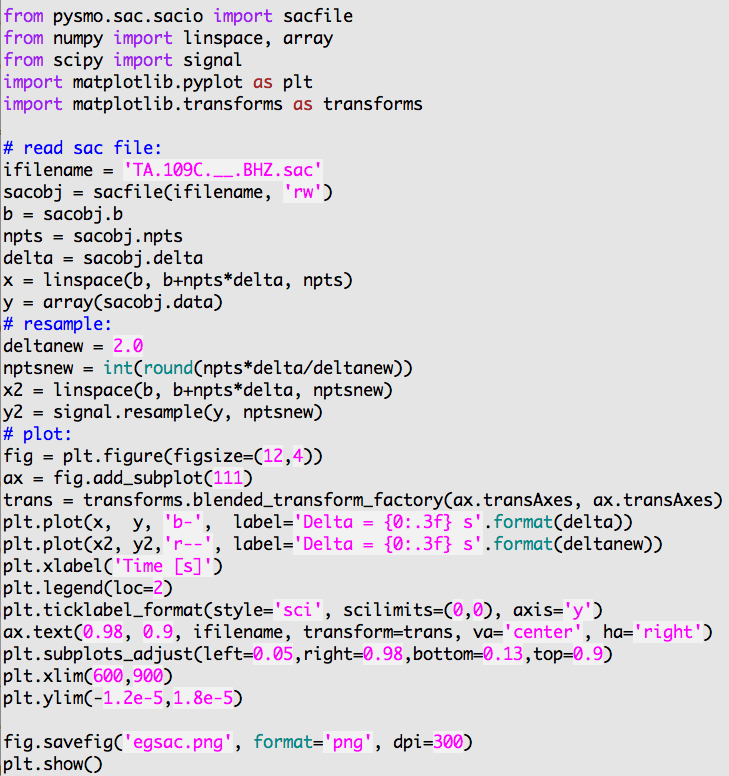
\includegraphics[width = 0.9 \textwidth]{figs/prog-egsac.png}
    \caption{The \texttt{<pkg-install-dir>/pysmo-aimbat-0.1.1/scripts/egsac.py} script which produces Figure \ref{fig:egsac}. }
    \label{fig:prog-egsac}
\end{figure}


In this example, a SAC file named \texttt{TA.109C.\_\_.BHZ.sac} is read in as a sacfile object.
The time array is calculated from SAC headers. 
The data array is resampled from interval 0.025 to 2.0 seconds using Scipy's signal processing module.
Result is displayed in Figure \ref{fig:egsac}.

Add the following codes to write the resampled seismogram to file \texttt{TA.109C.\_\_.BHZ.sac}:

\begin{lyxcode}
sacobj.delta = deltanew

sacobj.npts = nptsnew

sacobj.data = y2
\end{lyxcode}



\begin{figure}[!h]
    \centering
    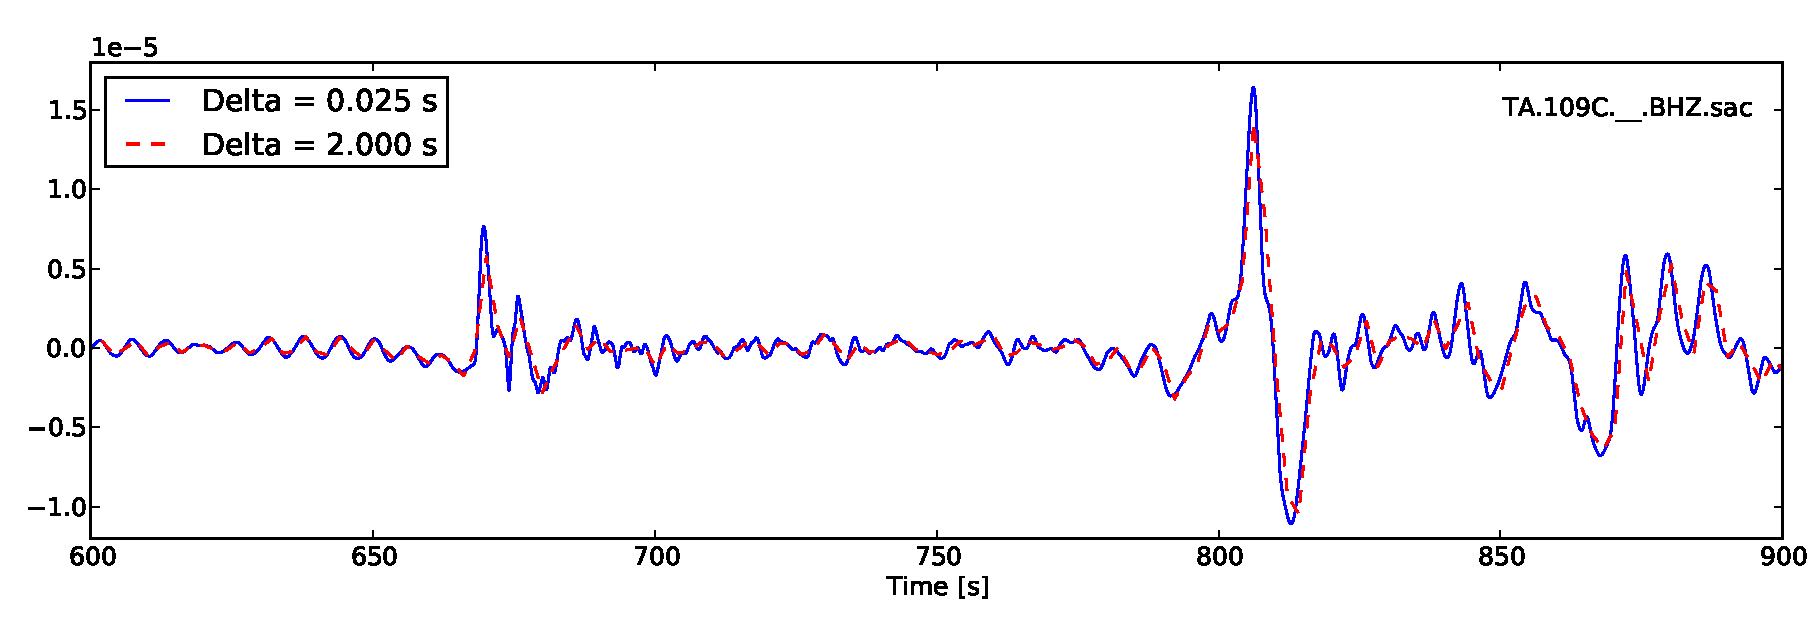
\includegraphics[width = 0.99 \textwidth]{figs/egsac-109c.pdf}
    \caption{Example of reading, resampling and plotting a SAC file. }
    \label{fig:egsac}
\end{figure}





\subsubsection{Python Pickle for SAC Files}

The \texttt{pysmo.sacio} module converts SAC files to \texttt{sacfile} objects. Any modification of the objects are instantly written to files. 
In data processing, the user may want to abandon changes made earlier, which brings the need of a buffer for the  \texttt{sacfile} objects.
The \texttt{SacDataHdrs} class in the \texttt{pysmo.aimbat.sacpickle} module is written on top of \texttt{pysmo.sacio} to serves this purpose by reading a SAC file and returning a \texttt{sacdh} object that is very similar of the \texttt{sacfile} object. 
Essentially, the \texttt{sacdh} object is a copy of the the \texttt{sacfile} object in the memory, except that SAC headers 't0-t9', 'user0-user9', 'kuser0-kuser2' are saved in three Python lists.
A \texttt{gsac} object of the \texttt{SacGroup} class consists of a group of \texttt{sacdh} objects from event-based SAC data files, earthquake hypocenter information and station locations.
An additional step is required to save changes in the \texttt{gsac} object to files.

In order to avoid frequent SAC file I/O, the \texttt{pickle/cPickle} module is used for serializing and de-serializing the \texttt{gsac} object structure.
Thus the data processing efficiency is improved because reading and writing of SAC files are done only once each before and after data processing.
Script \texttt{sac2pkl.py} does the conversions between SAC files and Python pickles. 
Its usage message can be printed out by running "\texttt{sac2pkl.py -h}" at command line and the result is displayed in Figure \ref{fig:help-sac2pkl}.
For example, in the data example directory \url{<example-event-dir>}, run

\begin{lyxcode}
sac2pkl.py -s *Z -o 20110915.19310408.bhz.pkl -d 0.025
\end{lyxcode}

to read 163 vertical component seismograms at a sample interval of 0.025 s and convert to a \texttt{gsac} object which is saved in the pickle file \texttt{20110915.19310408.bhz.pkl}.

To save disk space, compressed pickle files in gz and bz2 formats can be generated by:
\begin{lyxcode}
sac2pkl.py -s *Z -o 20110915.19310408.bhz.pkl -d 0.025 -z gz

sac2pkl.py -s *Z -o 20110915.19310408.bhz.pkl -d 0.025 -z bz2
\end{lyxcode}

at the cost of more CPU time.

After processing, run

\begin{lyxcode}
sac2pkl.py 20110915.19310408.bhz.pkl -p
\end{lyxcode}

to convert the pickle file to SAC files.

\begin{figure}[!h]
    \centering
    \vspace{1em}
    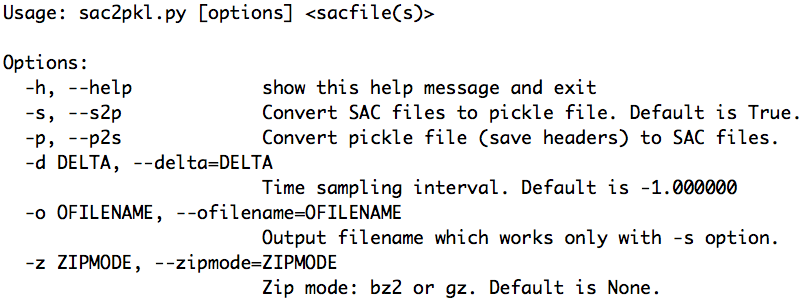
\includegraphics[width = 0.94 \textwidth]{figs/help-sac2pkl.png}
    \caption{Help message of the \texttt{sac2pkl.py} script. }
    \label{fig:help-sac2pkl}
\end{figure}

See the doc string of \texttt{pysmo.aimbat.sacpickle} (type "\texttt{from pysmo.aimbat import sacpickle; print sacpickle.\_\_doc\_\_}" in a Python shell) and 
\url{http://docs.python.org/library/pickle.html}
for more information about the Python data structure, pickling and unpickling.










%%%%%%%%%%%%%%%%%%%%%%%%%%%%
\subsection{SAC Plotting and Phase Picking}

\begin{figure}[!b]
    \centering
    \vspace{2em}
    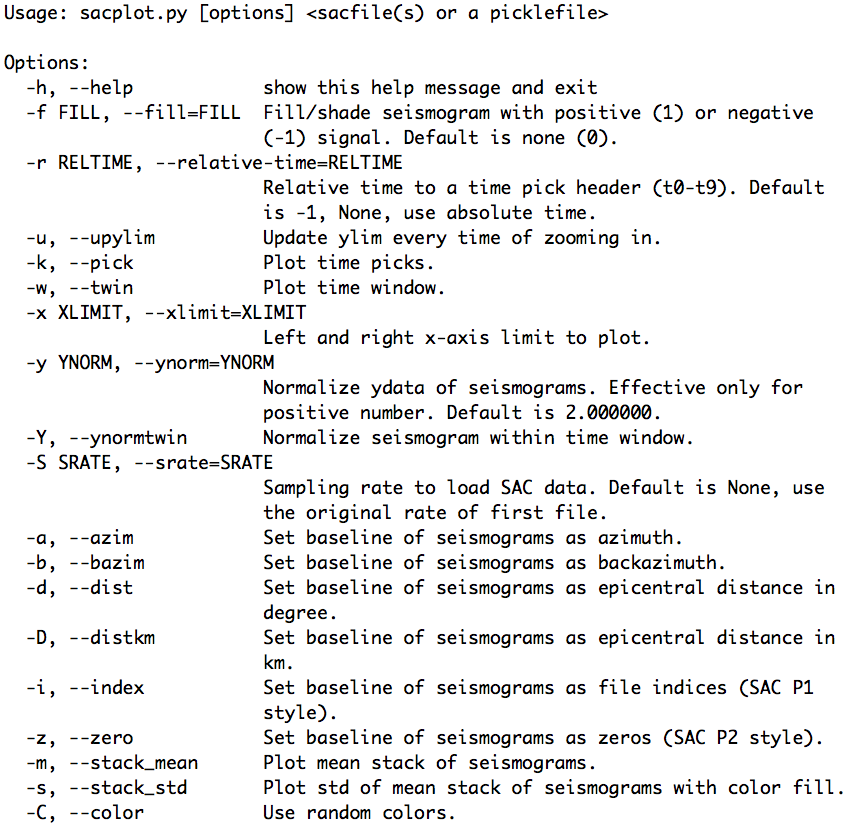
\includegraphics[width = 0.94 \textwidth]{figs/help-sacplot.png}
    \caption{Help message of the \texttt{sacplot.py} script. }
    \label{fig:help-sacplot}
\end{figure}


SAC plotting and phase picking functionalities are replicated and enhanced based on the GUI neutral widgets (such as Button and SpanSelector) and the event (keyboard and mouse events such as \texttt{key\_press\_event} and \texttt{mouse\_motion\_event}) handling API of Matplotlib \citep{matplotlib}.
They are implemented in two modules \texttt{pysmo.aimbat.plotphase} and \texttt{pysmo.aimbat.pickphase}, which are used by corresponding scripts \texttt{sacplot.py} and \texttt{sacppk.py} executable at command line. Their help messages are displayed in Figures \ref{fig:help-sacplot} and \ref{fig:help-sacppk}.



\begin{figure}[!h]
    \centering
    \vspace{1em}
    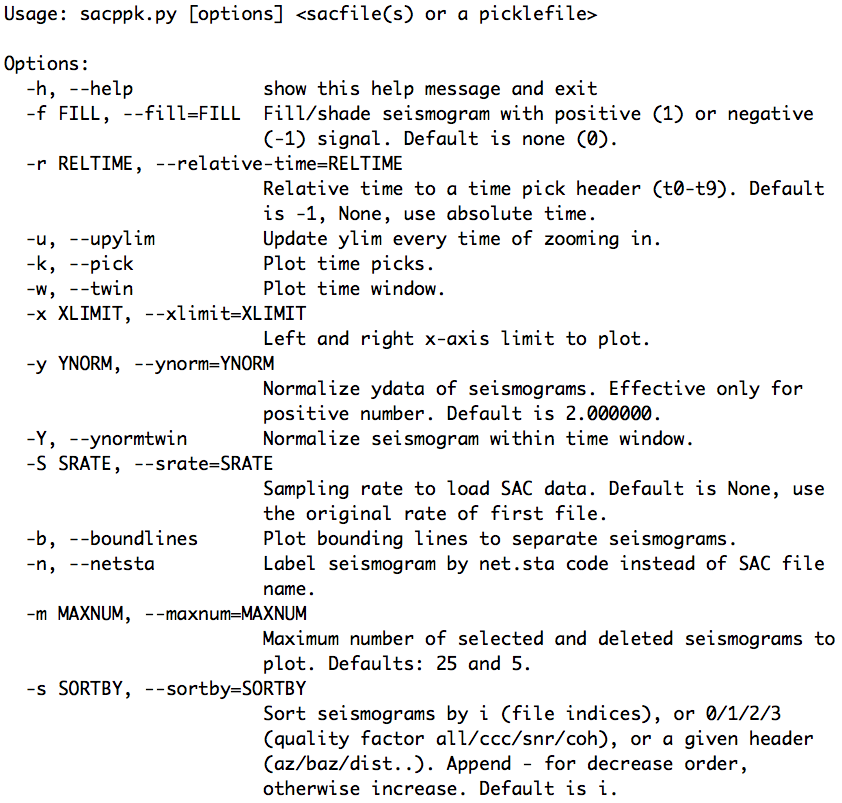
\includegraphics[width = 0.94 \textwidth]{figs/help-sacppk.png}
    \caption{Help message of the \texttt{sacppk.py} script. }
    \label{fig:help-sacppk}
\end{figure}



\begin{figure}[!h!b]
    \centering
    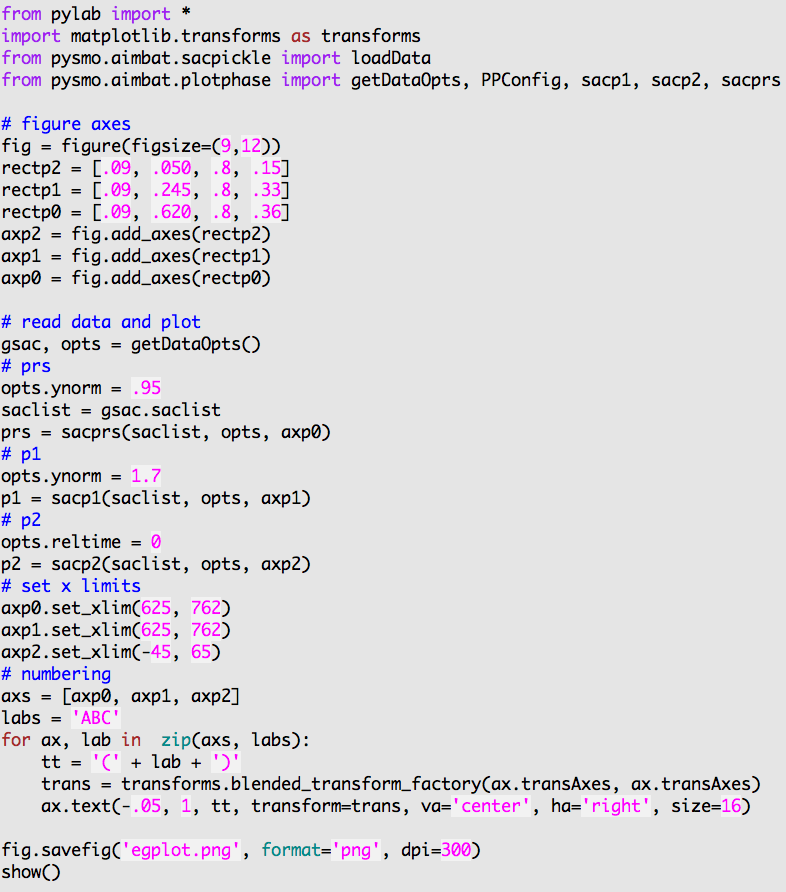
\includegraphics[width = 0.94 \textwidth]{figs/prog-egplot.png}
    \caption{The \texttt{<pkg-install-dir>/pysmo-aimbat-0.1.1/scripts/egplot.py} script which produces Figure \ref{fig:egplot}. }
    \label{fig:prog-egplot}
\end{figure}


\begin{figure}
    \centering
    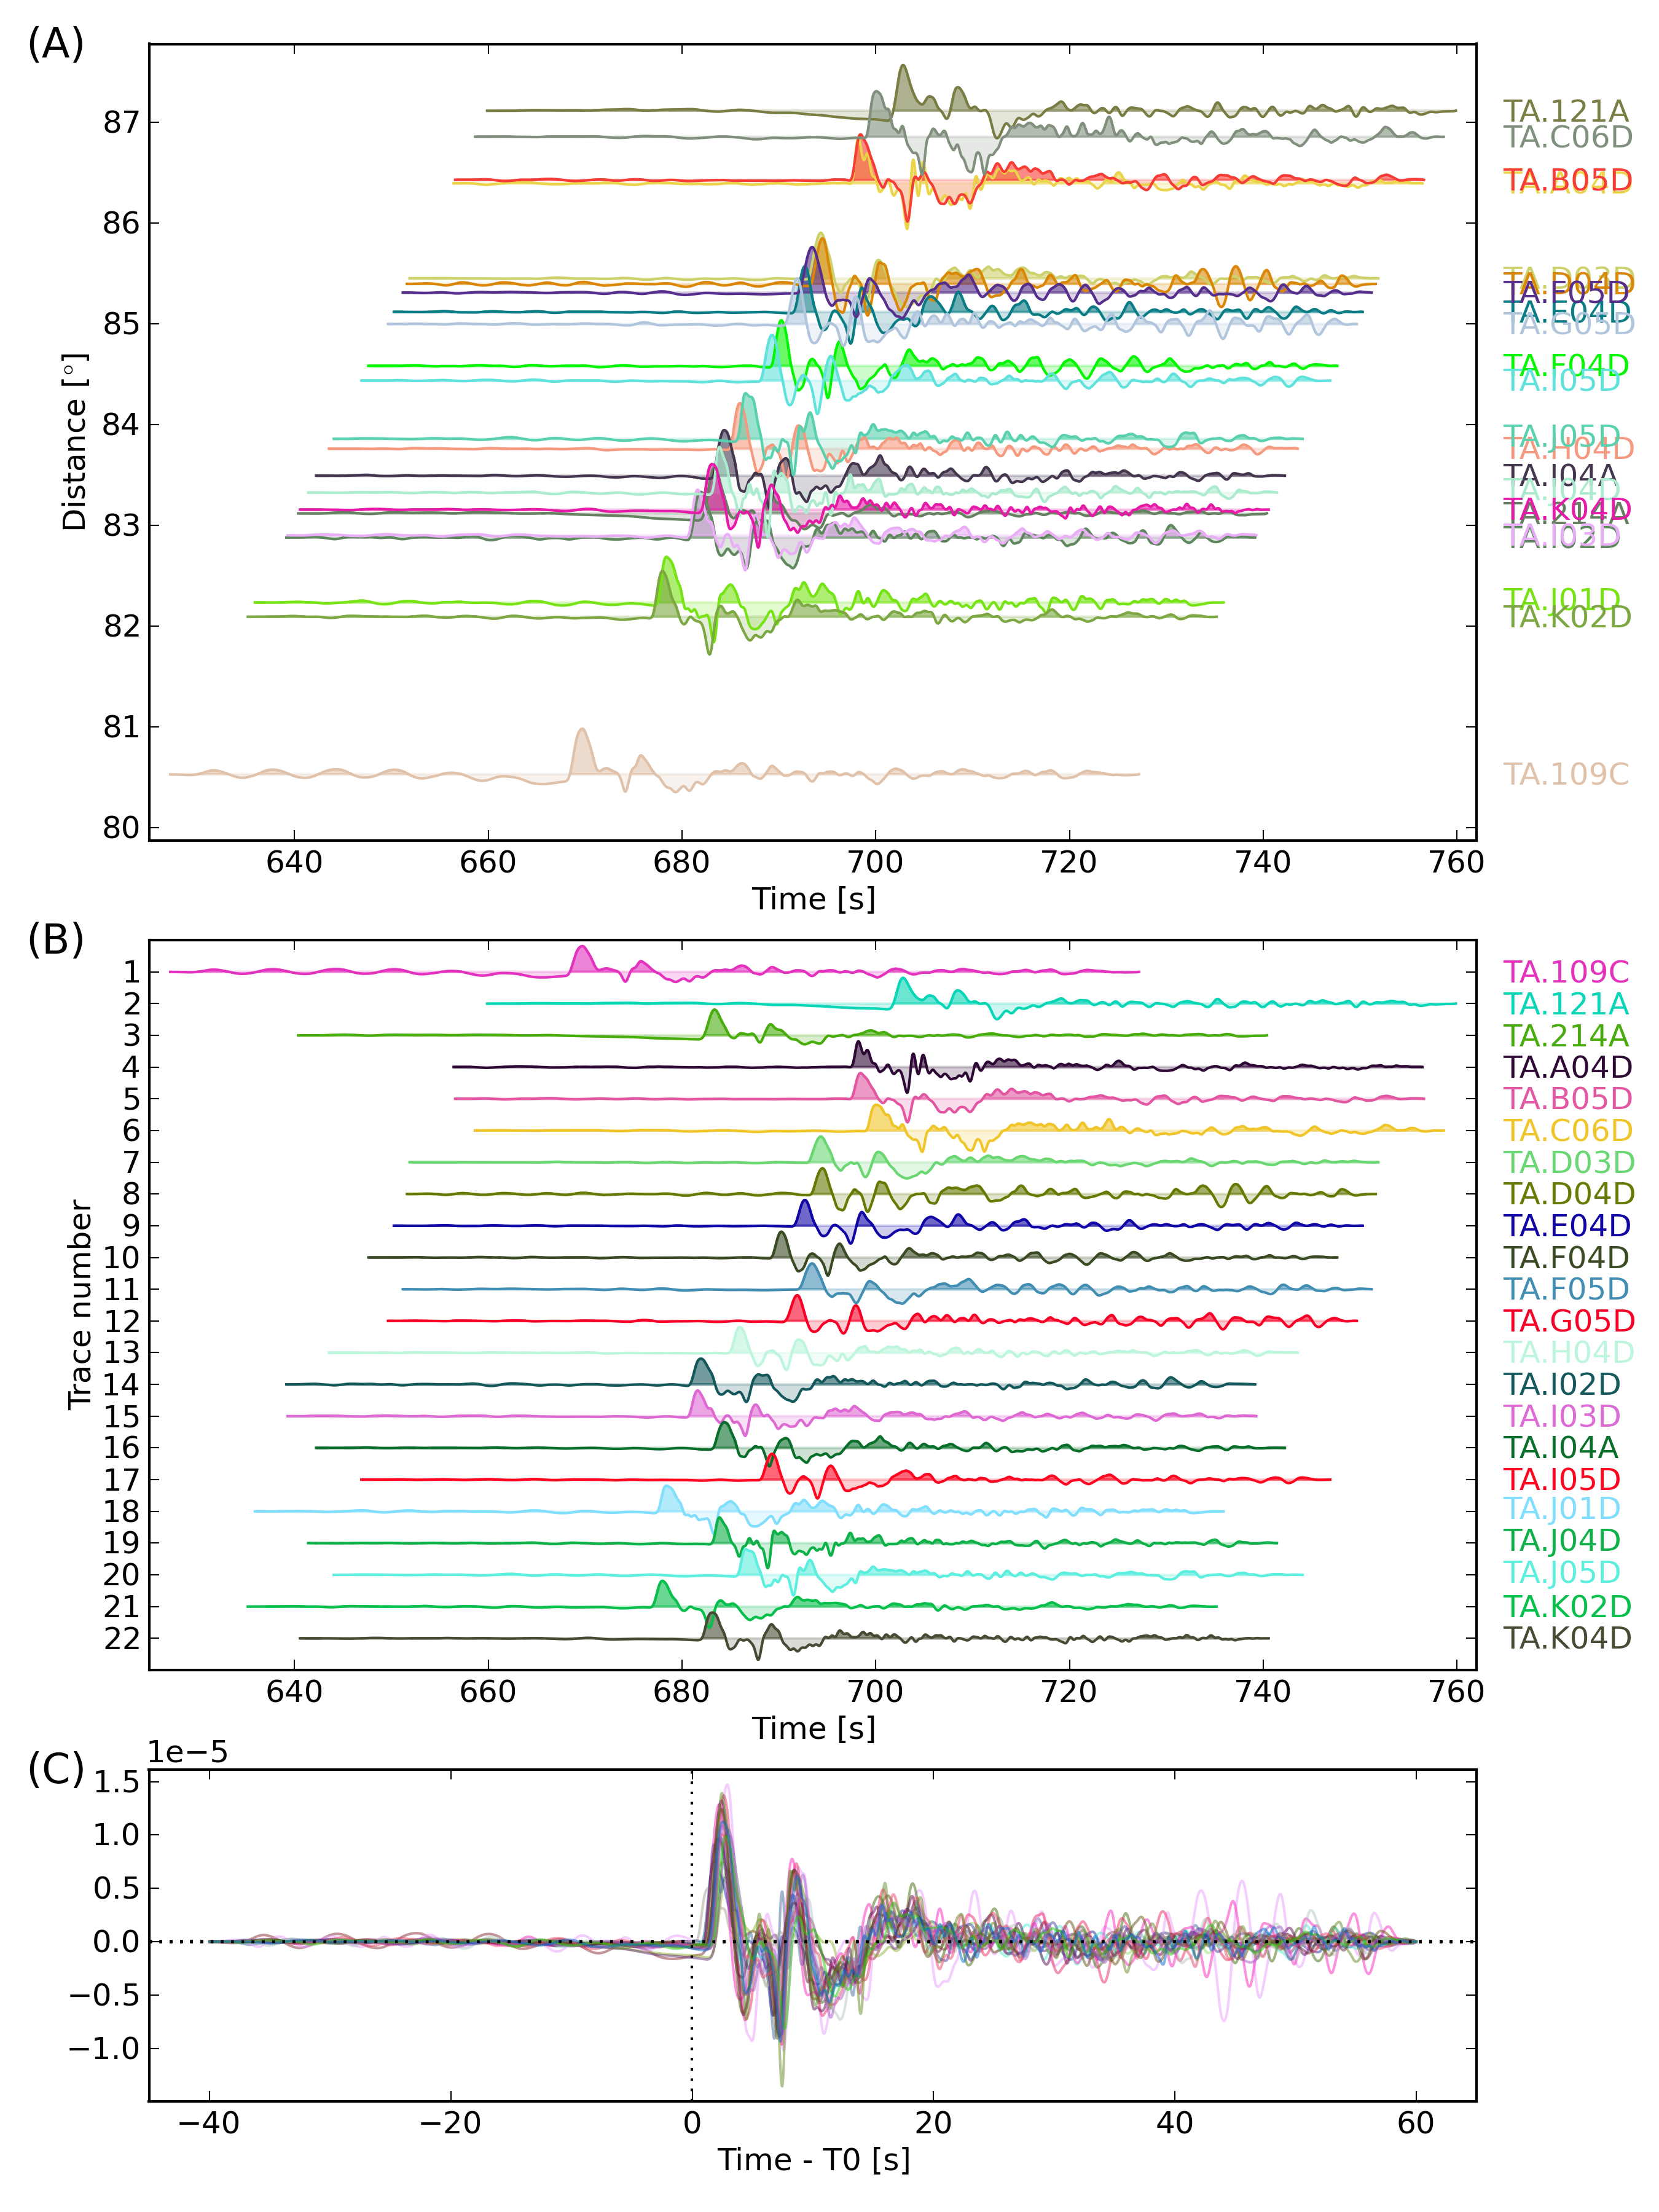
\includegraphics[width = 0.9 \textwidth]{figs/egplot.png}
    \caption{Example of plotting multiple SAC files in (A) record section; (B) SAC p1 style; and (C) SAC p2 style. 
    This figure is the random-color version of Figure 1 in \cite{pytool}. }
    \label{fig:egplot}
\end{figure}


%%%%%%%%%%%%%%% sacplot
\subsubsection{SAC Plotting}

Options "-i, -z, -d, -a, and -b" of \texttt{sacplot.py} set the seismogram plotting baseline as file index, zero, epicentral distance in degrees, azimuth, and back-azimuth, respectively. 
The user can run \texttt{sacplot.py} directly with the options, or run individual scripts
\texttt{sacp1.py}, \texttt{sacp2.py}, \texttt{sacprs.py}, \texttt{sacpaz.py}, and \texttt{sacpbaz.py} which preset the baseline options and plot seismograms in SAC p1 style, p2 style, record section, and relative to azimuth and back-azimuth. The following commands are equivalent:

\begin{lyxcode}
sacplot.py -i     $\Longleftrightarrow$   sacp1.py

sacplot.py -z    $\Longleftrightarrow$   sacp2.py

sacplot.py -d    $\Longleftrightarrow$   sacprs.py

sacplot.py -a    $\Longleftrightarrow$   sacpaz.py

sacplot.py -b    $\Longleftrightarrow$   sacpbaz.py

\end{lyxcode}


Input data files need to be supplied to the scripts in the form of either a list of SAC files or a pickle file which includes multiple SAC files. For example, a "bhz.pkl" file is generated from 22 vertical component seismograms "TA.[1-K]*Z" by running:

\begin{lyxcode}
sac2pkl.py TA.[1-K]*BHZ -o bhz.pkl -d0.025
\end{lyxcode}

in the data example directory \url{<example-event-dir>}. Then the two commands are equivalent:

\begin{lyxcode}
sacp1.py TA.[1-K]*Z    $\Longleftrightarrow$   sacp1.py bhz.pkl
\end{lyxcode}

For large number of seismograms, the pickle file is suggested because of faster loading.


Besides using the standard \texttt{sacplot.py} script, the user can modify its \texttt{getAxes} function in your own script to customize figure size and axes attributes.
Script \texttt{egplot.py} (Figure \ref{fig:prog-egplot}) is such an example in which SAC p1, p2 styles and record section plotting are drawn in three axes in the same figure canvas. Run

\begin{lyxcode}
egplot.py TA.[1-K]*Z  -f1 -C
\end{lyxcode}

at command line to produce Figure \ref{fig:egplot}.
The "-C" option uses random color for each seismogram.
The "-f1" option fills the positive signals of waveform with less transparency.  
In the script, "opts.ynorm" sets the waveform normalization and "opts.reltime=0" sets the time axis relative to time pick t0.


An improvement over SAC is that the program outputs the filename when the seismogram is clicked on by the mouse. This is enabled by the event handling API and is mostly introduced for use in SAC p2 style plotting when seismograms are plotted on top of each other. It is especially useful when a large number of seismograms create difficulties in labeling.

Another improvement is easier window zooming enabled by the SpanSelector widget and the event handling API.
Select a time span by mouse clicking and dragging to zoom in a waveform section.
Press the 'z' key to zoom out to the previous time range.




%%%%%%%%%%%%%%% sacppk

\subsubsection{SAC Phase Picking}

SAC plotting (\texttt{pysmo.aimbat.plotphase}) does not involve change in data files but phase picking (\texttt{pysmo.aimbat.pickphase}) does.
A GUI is built for user to interactively pick phase arrival times. 
Figure \ref{fig:sacppk} is an example screen shot running

\begin{lyxcode}
sacppk.py 20110915.19310408.bhz.pkl -w
\end{lyxcode}

in the data example directory \url{<example-event-dir>}.


\begin{figure}[!hb]
    \centering
    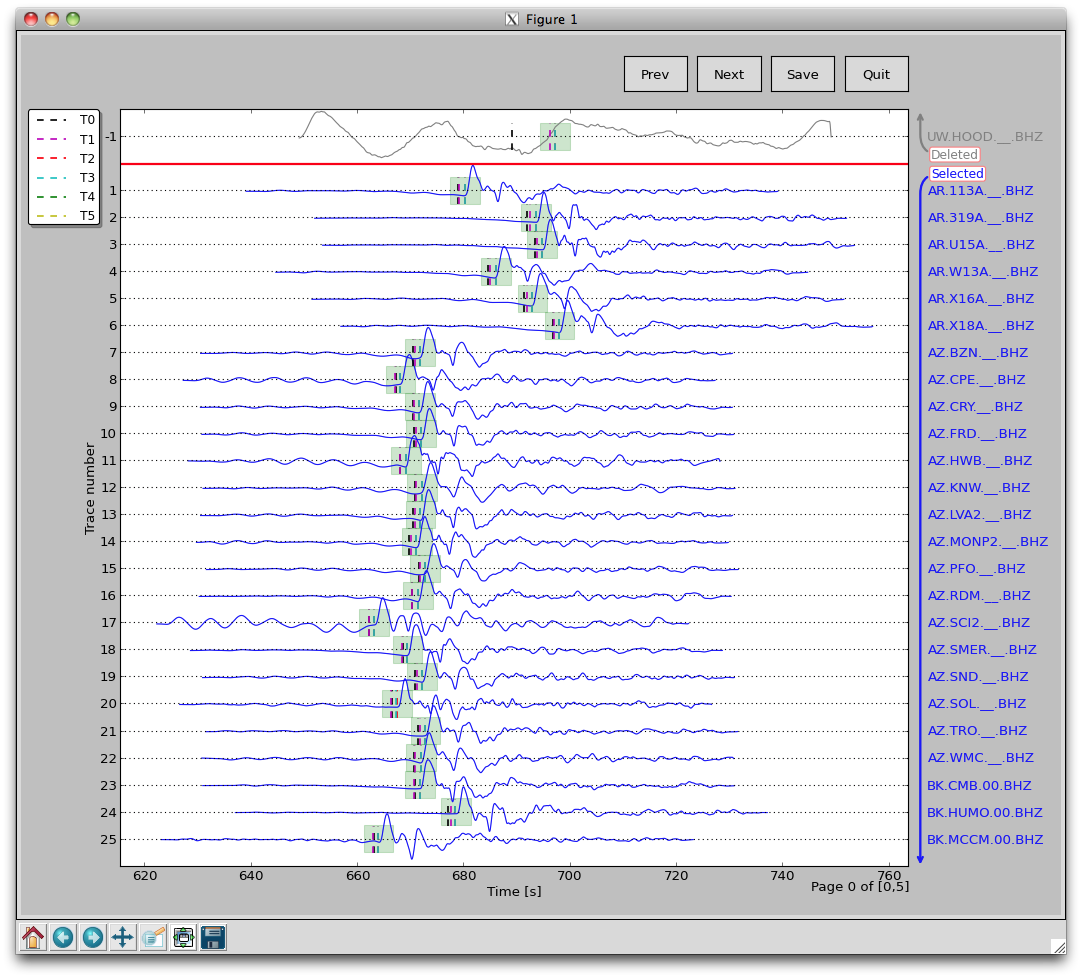
\includegraphics[width = 0.94 \textwidth]{figs/sacppk.png}
    \caption{Screen shot of running "\texttt{sacppk.py 20110915.19310408.bhz.pkl -w}". 
    First 25 out 162 selected seismograms and 1 deleted seismogram are plotted on the first page. 
    Click the \texttt{Prev} and \texttt{Next} Buttons to navigate through the total 6 pages. 
    }
    \label{fig:sacppk}
\end{figure}


Following SAC convention, the user can set a time pick by pressing the 't' key and number keys '0-9'. The x location of the mouse position is saved to corresponding SAC headers 't0-t9'. 
Time window zooming in \texttt{pysmo.aimbat.pickphase} is implemented in the same way as in \texttt{pysmo.aimbat.plotphase} to replace SAC's combination of the 'x' key and mouse click. 
Zooming out key is set to 'z' because the 'o' key is used for another purpose by Matplotlib.
The filename printing out by mouse clicking feature is also available in \texttt{pysmo.aimbat.pickphase}.

A major improvement over SAC is picking a time window in addition to time picks.
Pressing the 'w' key to save the current time axis range to two user-defined SAC header variables. A transparent green span is plotted within the time window (Figure \ref{fig:sacppk}).

Another major improvement involves quality control with convenient operations to (de)select seismograms.
In the GUI in Figure \ref{fig:sacppk}, there are two divisions of selected and deleted seismograms. 
Selected seismograms with a positive trace number are displayed with blue wiggles, while deleted seismograms with negative trace numbers are plotted in gray.
The user can simply click on a certain seismogram to switch the selection status, either to exclude it or bring it back for inclusion. The trace selection status is stored in a user-defined SAC header variable.

In SAC, command "ppk p 10" plots 10 seismograms on each page. Pressing the 'b' and 'n' keys to navigate through pages.
The number of seismograms plotted on each page is controlled by command line option "-m maxsel maxdel" for \texttt{sacppk.py}. The \texttt{Prev} and \texttt{Next} Buttons are for page navigation and the \texttt{Save} Button saves the change in time picks and time window to files.
The default values for maxsel and maxdel are 25 and 5, which means a maximum of 30 seismograms on each page. 
In Figure \ref{fig:sacppk}, there are 26 seismograms on the first page because only 1 seismogram is deleted. 
On next page, there are 30 selected seismograms. To plot 50 seismograms on each page, run


\begin{lyxcode}
sacppk.py 20110915.19310408.bhz.pkl -w -m 45 5
\end{lyxcode}

and there would be 4 total pages and 13 seismograms on the last page.


To plot seismograms relative to time pick t0 and fill the positive and negative wiggles of waveform, run

\begin{lyxcode}
sacppk.py 20110915.19310408.bhz.pkl -w -r0 -f1
\end{lyxcode}

To sort seismograms by epicentral distance in increase and decrease orders, run

\begin{lyxcode}
sacppk.py 20110915.19310408.bhz.pkl -w -sdist

sacppk.py 20110915.19310408.bhz.pkl -w -sdist-
\end{lyxcode}

Sorting by azimuth and back-azimuth is similar:
\begin{lyxcode}
sacppk.py 20110915.19310408.bhz.pkl -w -saz

sacppk.py 20110915.19310408.bhz.pkl -w -sbaz
\end{lyxcode}






\begin{figure}[!b]
    \centering
    \vspace{2em}
    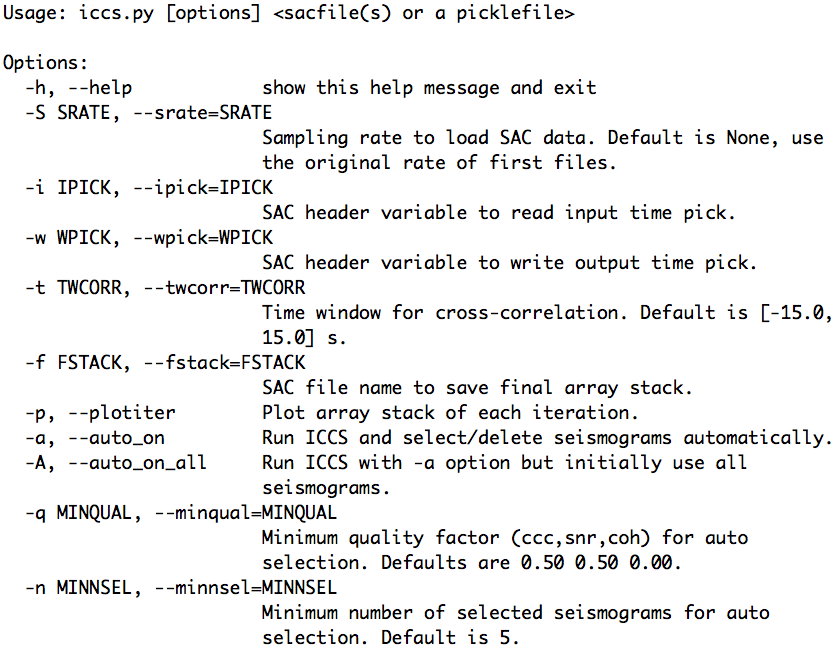
\includegraphics[width = 0.94 \textwidth]{figs/help-iccs.png}
    \caption{Help message of the \texttt{iccs.py} script. }
    \label{fig:help-iccs}
\end{figure}

\begin{figure}[!b]
    \centering
    \vspace{2em}
    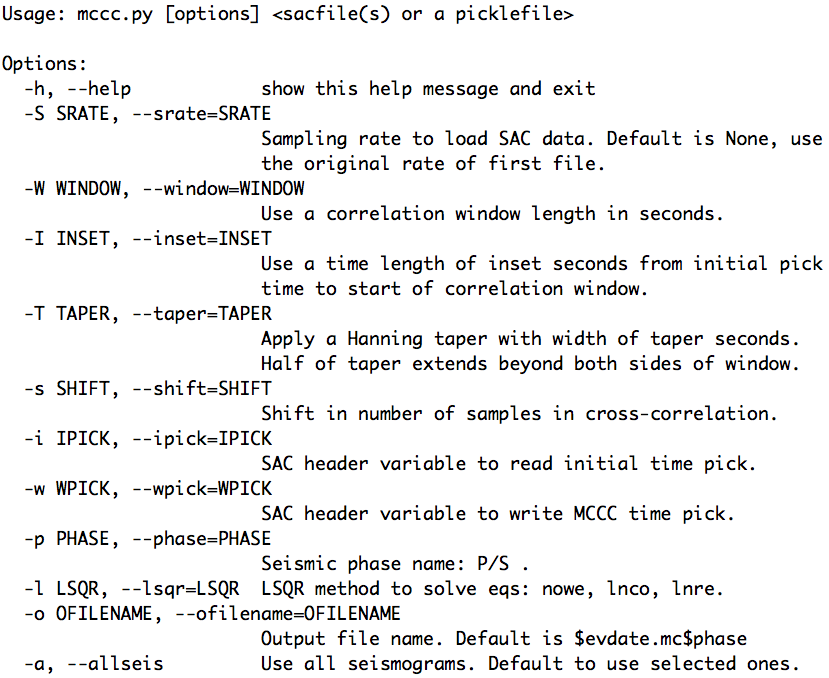
\includegraphics[width = 0.94 \textwidth]{figs/help-mccc.png}
    \caption{Help message of the \texttt{mccc.py} script. }
    \label{fig:help-mccc}
\end{figure}


%%%%%%%%%%%%%%%%%%%%%%%%%%%%
\newpage
\subsection{Measuring Teleseismic Body Wave Arrival Times}

The core idea in using AIMBAT to measure teleseismic body wave arrival times has two parts: automated phase alignment and interactive quality control. 
The first part reduces user processing time and the second part retains valuable user inputs.


\subsubsection{Automated Phase Alignment}

The ICCS algorithm calculates an array stack from predicted time picks, cross-correlates each seismogram with the array stack to find the time lags at maximum cross-correlation, then use the new time picks to update the array stack in an iterative process. 
The MCCC algorithm cross-correlates each possible pair of seismograms and uses a least-squares method to calculate an optimized set of relative arrival times.
Our method is to combine ICCS and MCCC in a four-step procedure using four anchoring time picks $_0T_i$, $_1T_i$, $_2T_i$, and $_3T_i$:
\begin{enumerate}[(a)]
\item \label{stepa} Coarse alignment by ICCS
\item \label{stepb} Pick phase arrival at the array stack
\item \label{stepc} Refined alignment by ICCS 
\item \label{stepd} Final alignment by MCCC
\end{enumerate}

The input and output time picks for the steps (a), (c) and (d) and their corresponding SAC headers are listed in Table \ref{table:steps}.
The one-time manual phase picking at the array stack in step (b) allows the measurement of absolute arrival times.
The detailed methodology and procedure can be found in \cite{pytool}. 

%%%%%%%
\begin{table}[!h]
\centering
{%\footnotesize
\scriptsize
\begin{tabular}{c c c c c c c }
\toprule
\multirow{3}*{Step} &	\multirow{3}*{Algorithm} 	&	\multicolumn{3}{c}{Input}		&	\multicolumn{2}{c}{Output}	\\
\cmidrule(l){3-5}  \cmidrule(l){6-7} \\
&&Time Window & Time Pick & Time Header	& Time Pick & Time Header \\
\midrule
(a)		&	ICCS			&	$W_a$			&	$_0T_i$	&	\textbf{T0}	&	$_1T_i$ 	&	\textbf{T1}		\\
(c)		&	ICCS			&	$W_b$			&	$_2T_i'$	&	\textbf{T2}	&	$_2T_i$ 	&	\textbf{T2}		\\
(d)		&	MCCC		&	$W_b$			&	$_2T_i$	&	\textbf{T2}	&	$_3T_i$ 	&	\textbf{T3}		\\
\bottomrule
\end{tabular}
}
\caption{Time picks and their SAC headers used in the procedure for measuring teleseismic body wave arrival times.
} 
\label{table:steps}
\end{table} 
%%%%%%%



The ICCS and MCCC algorithms are implemented in two modules \texttt{pysmo.aimbat.algiccs} and \texttt{pysmo.aimbat.algmccc}, and can be executed in scripts \texttt{iccs.py} and \texttt{mccc.py}, respectively. Usages are displayed in Figures \ref{fig:help-iccs} and  \ref{fig:help-mccc}.



\subsubsection{Interactive Quality Control and Graphical User Interface}

In practical data processing, there is a constant need of seismogram quality control, which is mixed with the procedure described above. ICCS steps (a), (b), and (c) are likely to be applied multiple times after removing low quality seismograms.
To facilitate quality control, ICCS calculates three quality factors for each seismogram: cross-correlation coefficient (CCC), signal-to-noise ratio (SNR), and time domain coherence (COH).
The "-a" and "-A" modes of \texttt{iccs.py} can remove seismograms with low qualities and rerun ICCS until all seismograms meet the minimum requirements specified by the "-q" option.

A GUI is also designed to run both ICCS and MCCC and perform interactive quality control. It is implemented in module \texttt{pysmo.aimbat.qualctrl} and script \texttt{ttpick.py} based on \texttt{pysmo.aimbat.pickphase} and four Buttons for the four-step procedure.
The quality control operation is the same as \texttt{sacppk.py}. The user can interactively switch the selection status of a seismogram by mouse clicking on the waveform. 
In order to efficiently delete low quality seismograms, different attributes listed below are used as sorting criteria:
\begin{itemize}
  \item -s 0: sort by user-defined weighted-average of CCC, SNR and COH
  \item -s 1: sort by CCC
  \item -s 2: sort by SNR
  \item -s 3: sort by COH
  \item -s t: sort by time pick difference
  \item -s az: sort by azimuth
  \item -s baz: sort by back-azimuth
  \item -s dist: sort by epicentral distance
\end{itemize}
Other SAC headers also work with the "-s" option.
Default sorting order is increase. Append "-" to make it decrease order, such as "-s t-".
Sorting by time pick difference (${_2}T_i-{_0}T_i$) in both increase and decrease orders are useful in detecting cycle-skipping.



\begin{figure}[!hb]
    \centering
    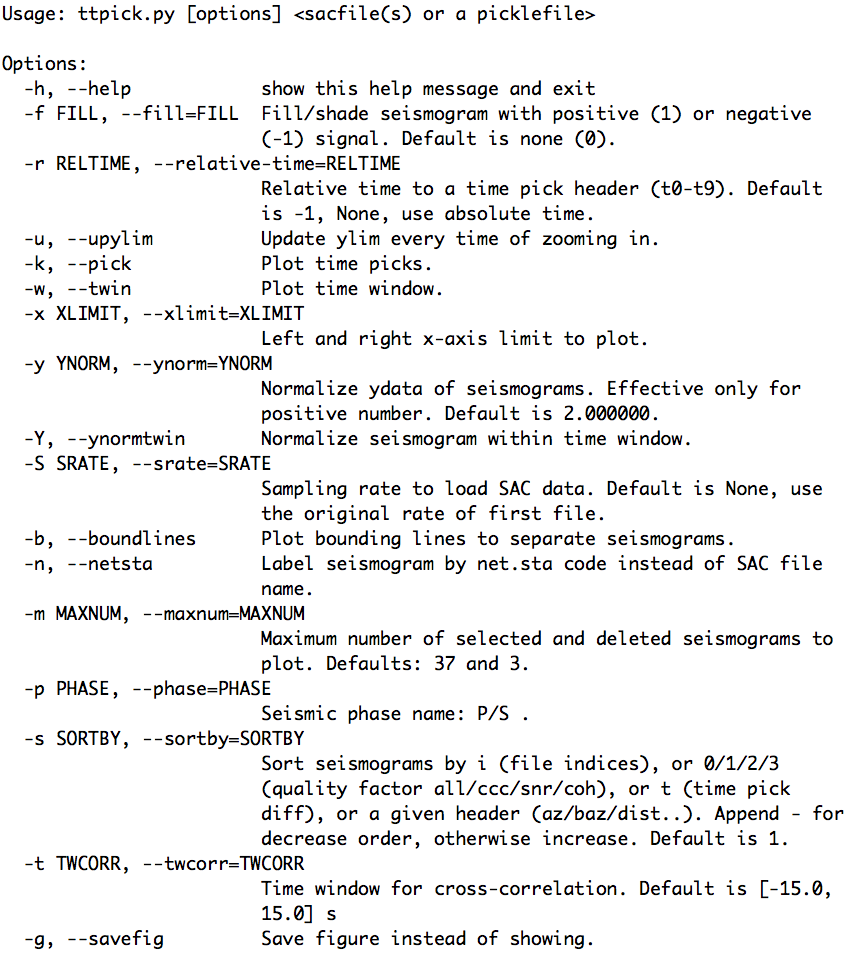
\includegraphics[width = 0.94 \textwidth]{figs/help-ttpick.png}
    \caption{Help message of the \texttt{ttpick.py} script. }
    \label{fig:help-ttpick}
\end{figure}



To start the GUI, run 

\begin{lyxcode}
ttpick.py 20110915.19310408.bhz.pkl -t -10 10 -s1
\end{lyxcode}

in the data example directory \url{<example-event-dir>} and the screen shot is displayed in Figure \ref{fig:ttpicka}.
The "-t -10 10" option specifies an initial time window of (-10,10) seconds around the initial time pick to run ICCS.
More screen shots along the data processing workflow are shown in Figures \ref{fig:ttpick1}-\ref{fig:ttpick4}. See the captions for commands and descriptions.







\begin{figure}[!h]
    \centering
    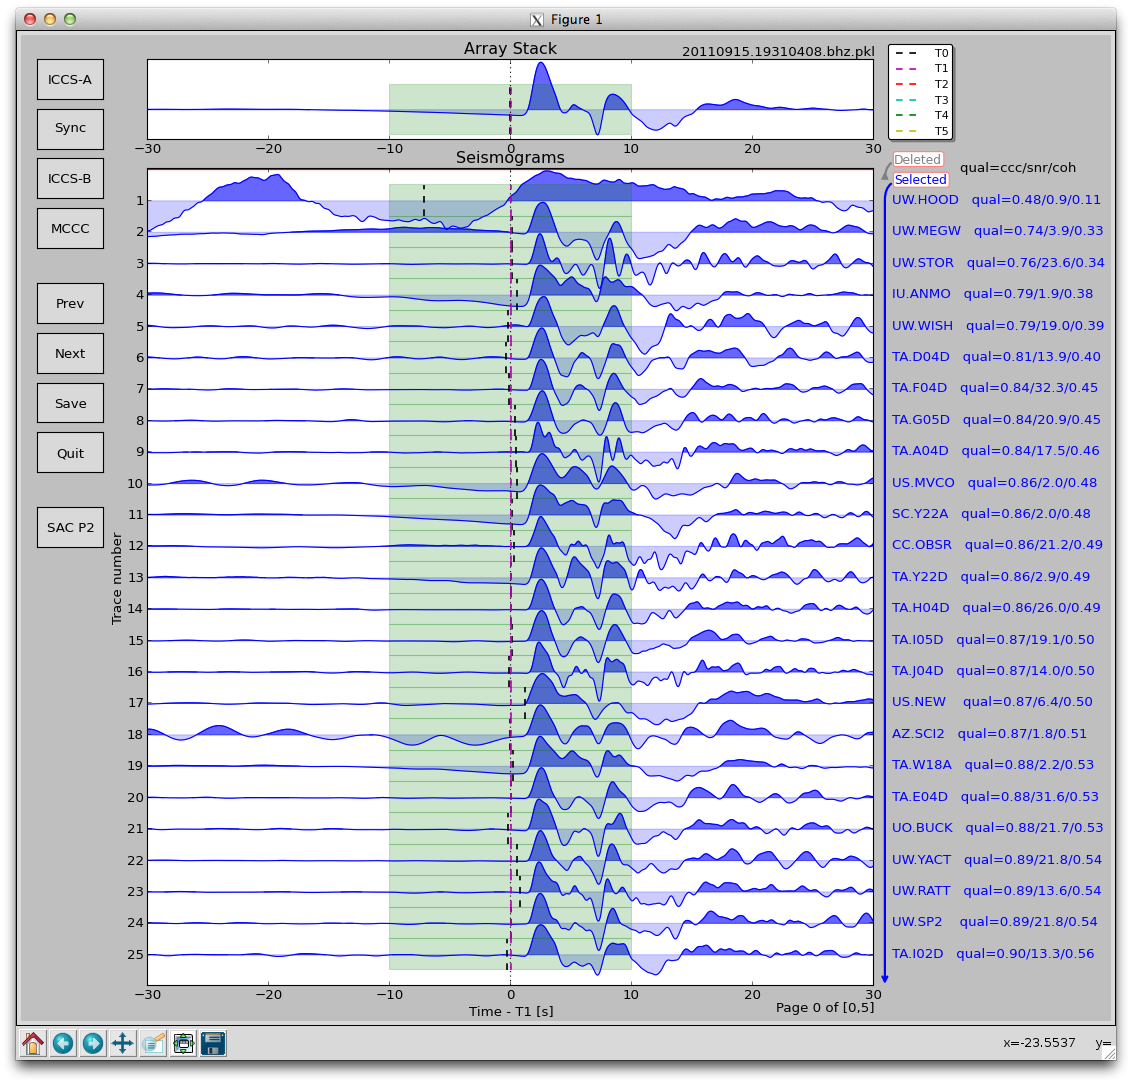
\includegraphics[width = 0.94 \textwidth]{figs/snapshots/ttpick-r1-s1-all.png}
    \caption{Screen shot of data processing initiated by running command \texttt{"ttpick.py 20110915.19310408.bhz.pkl -t -10 10 -s1 -x -30 30"}. Initial time window $W_a= (-10, 10)$ s. The "-x -30 30" option sets the time axis range to be (-30, 30) s. Seismograms are sorted by CCC.
    }
    \label{fig:ttpicka}
\end{figure}



\begin{figure}[!h]
    \centering
    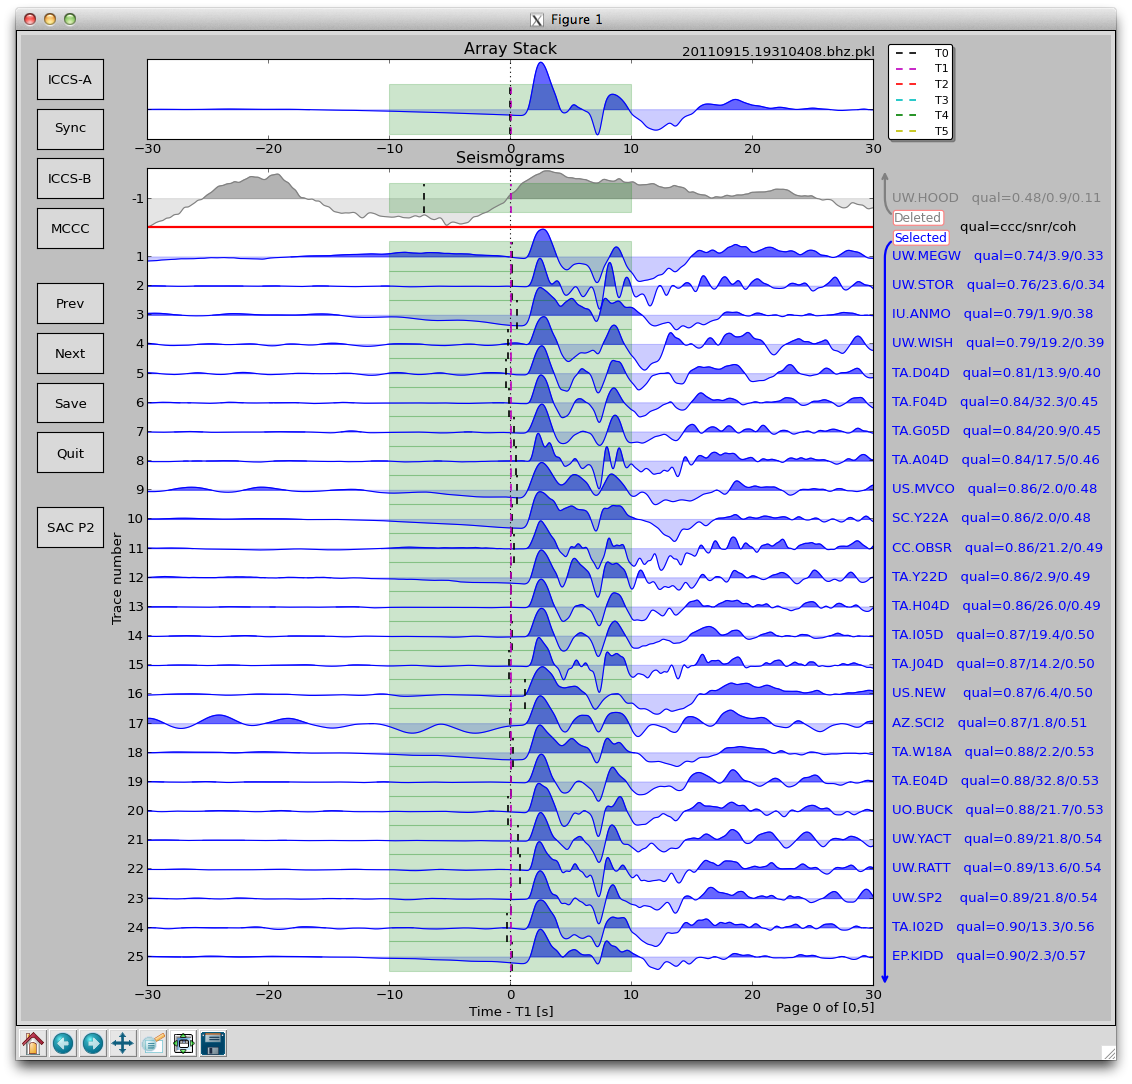
\includegraphics[width = 0.494 \textwidth]{figs/snapshots/ttpick-r1-s1-rerun.png}
    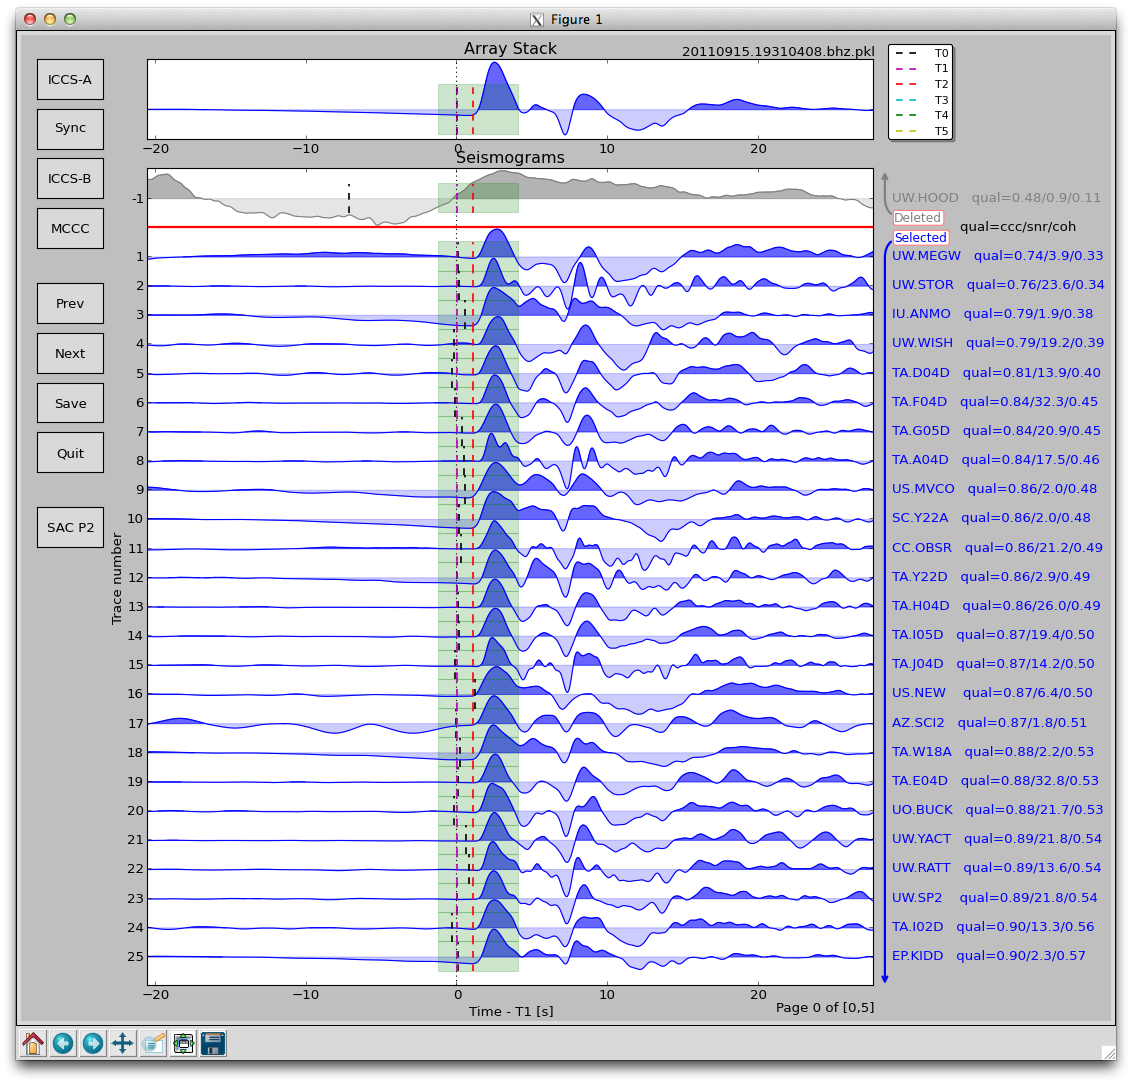
\includegraphics[width = 0.494 \textwidth]{figs/snapshots/ttpick-r1-s1-sync.png}
    \caption{
    (A) Delete station UW.WOOD and rerun ICCS step (a) by clicking the \texttt{ICCS-A} Button.
    (B) Pick phase emergence on the array stack for measuring absolute arrival times. Choose a smaller time window $W_b=(-2.7, 2.9)$ s for refined alignment. Click the \texttt{Sync} Button to get $_2T_i'$ and time window for each seismogram.
    }
    \label{fig:ttpick1}
\end{figure}


\begin{figure}[!h]
    \centering
        \vspace{3em}
    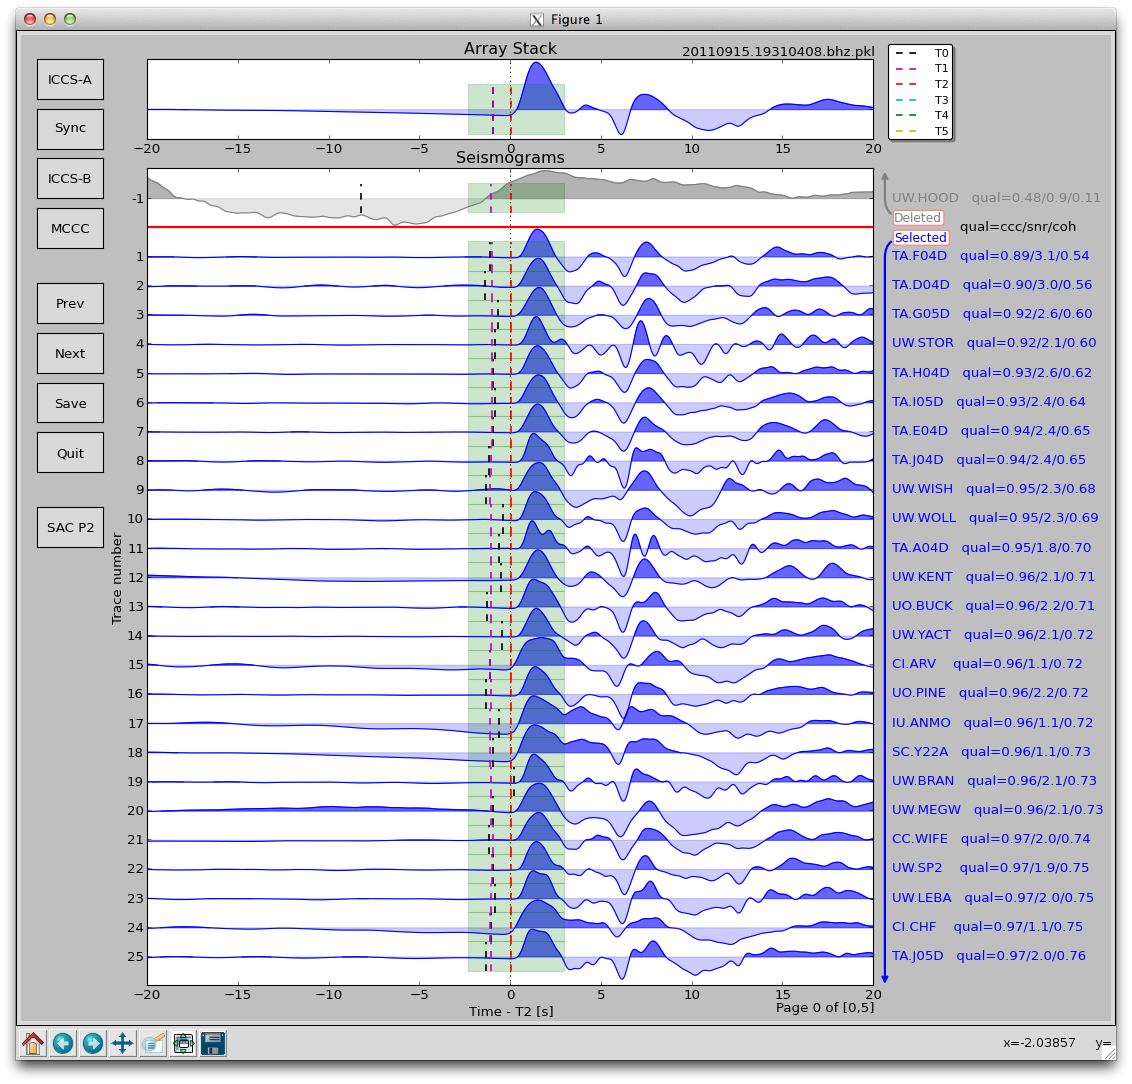
\includegraphics[width = 0.494 \textwidth]{figs/snapshots/ttpick-r2-s1.png}
    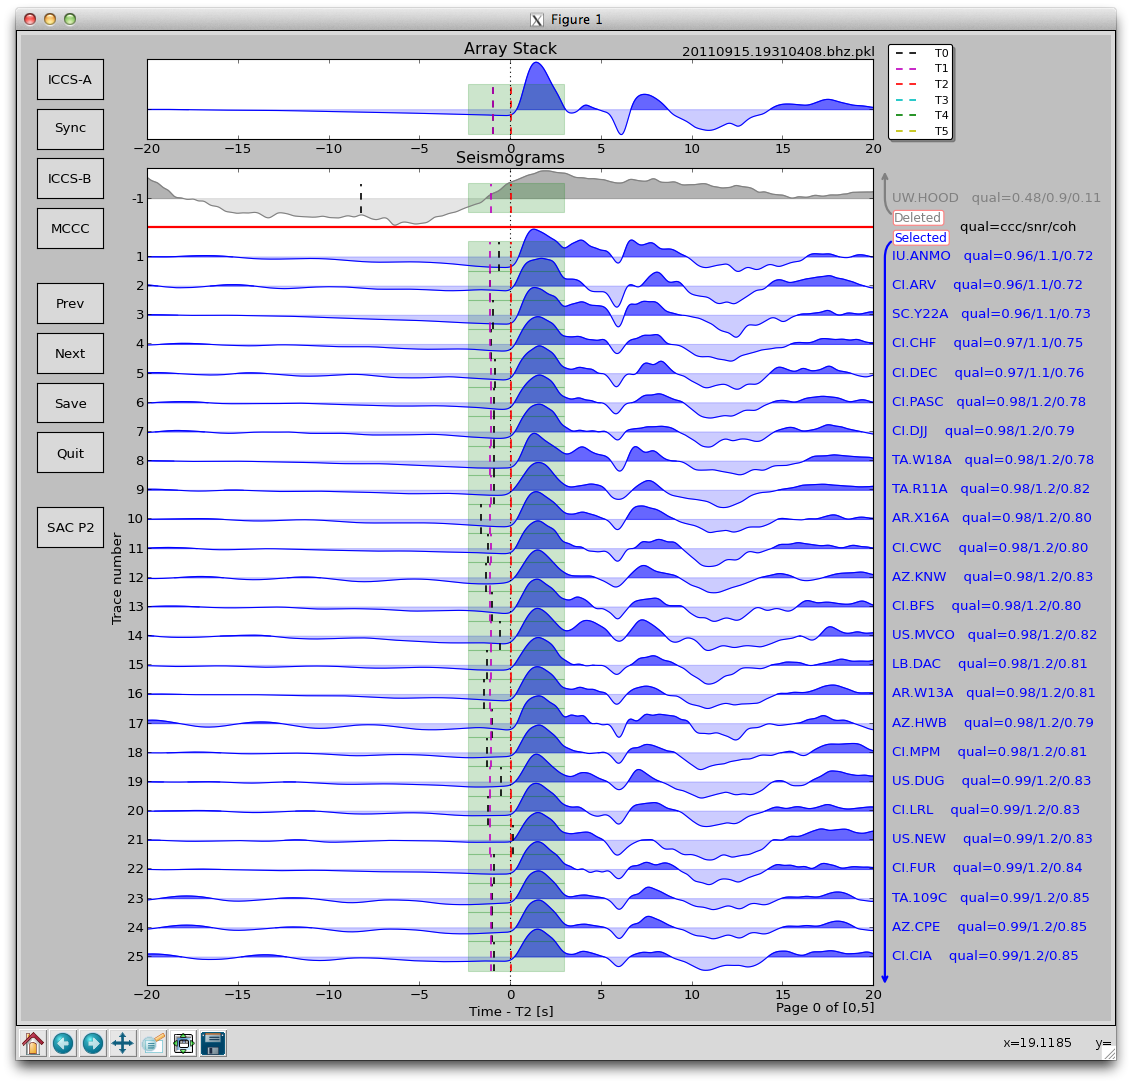
\includegraphics[width = 0.494 \textwidth]{figs/snapshots/ttpick-r2-s0.png}
    \caption{
    (A) Run ICCS step (c) by clicking the \texttt{ICCS-B} Button. Relative time pick is changed from T1 to T2.
    (B) Quit GUI and restart with \texttt{"ttpick.py 20110915.19310408.bhz.pkl -x -20 20 -r2 -s0"} which sorts seismograms by weighted-average of three quality factors. 
    }
    \label{fig:ttpick2}
\end{figure}


\begin{figure}[!h]
    \centering
    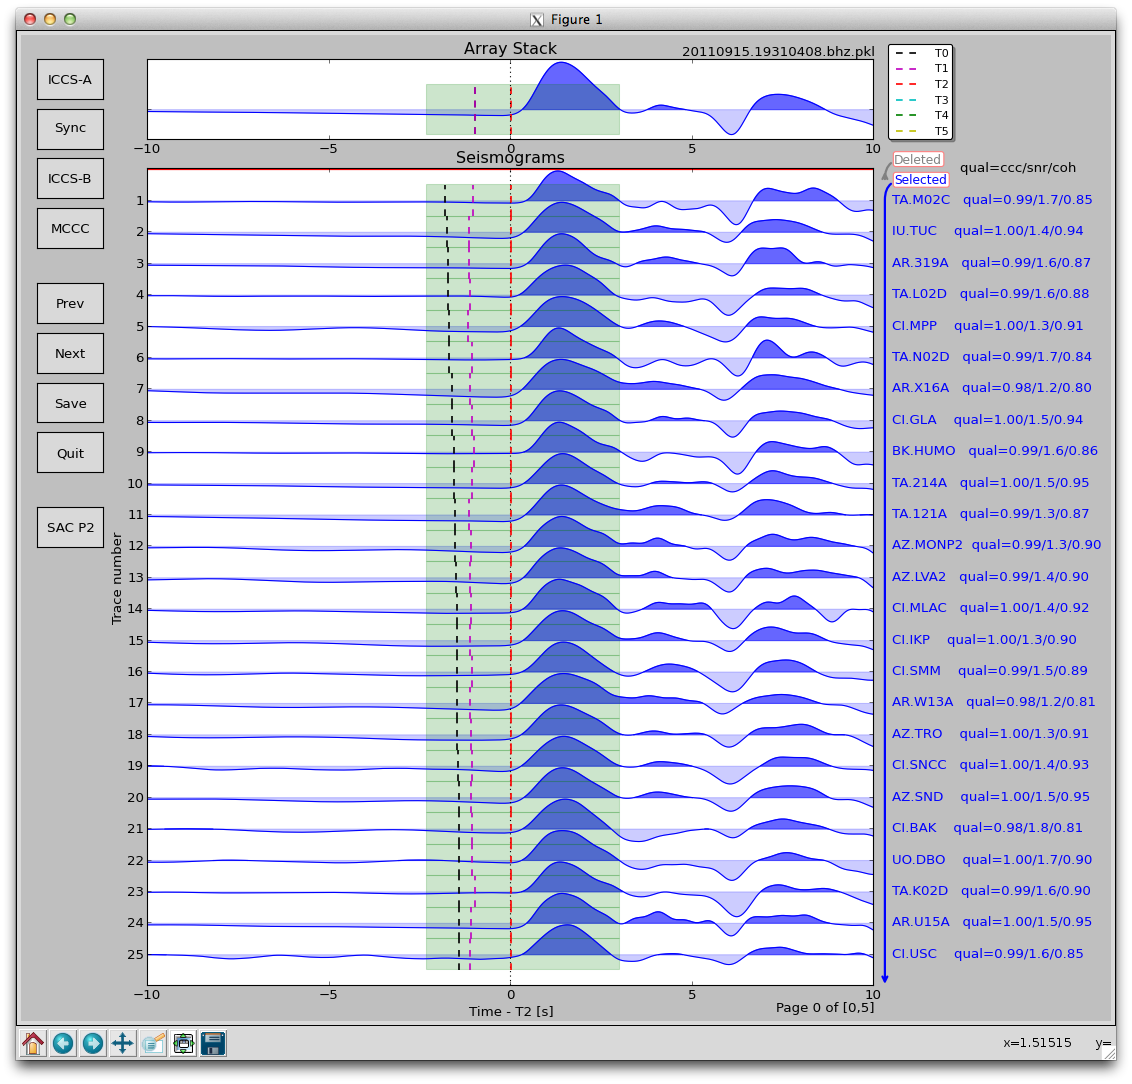
\includegraphics[width = 0.494 \textwidth]{figs/snapshots/ttpick-r2-st-decrease.png}
    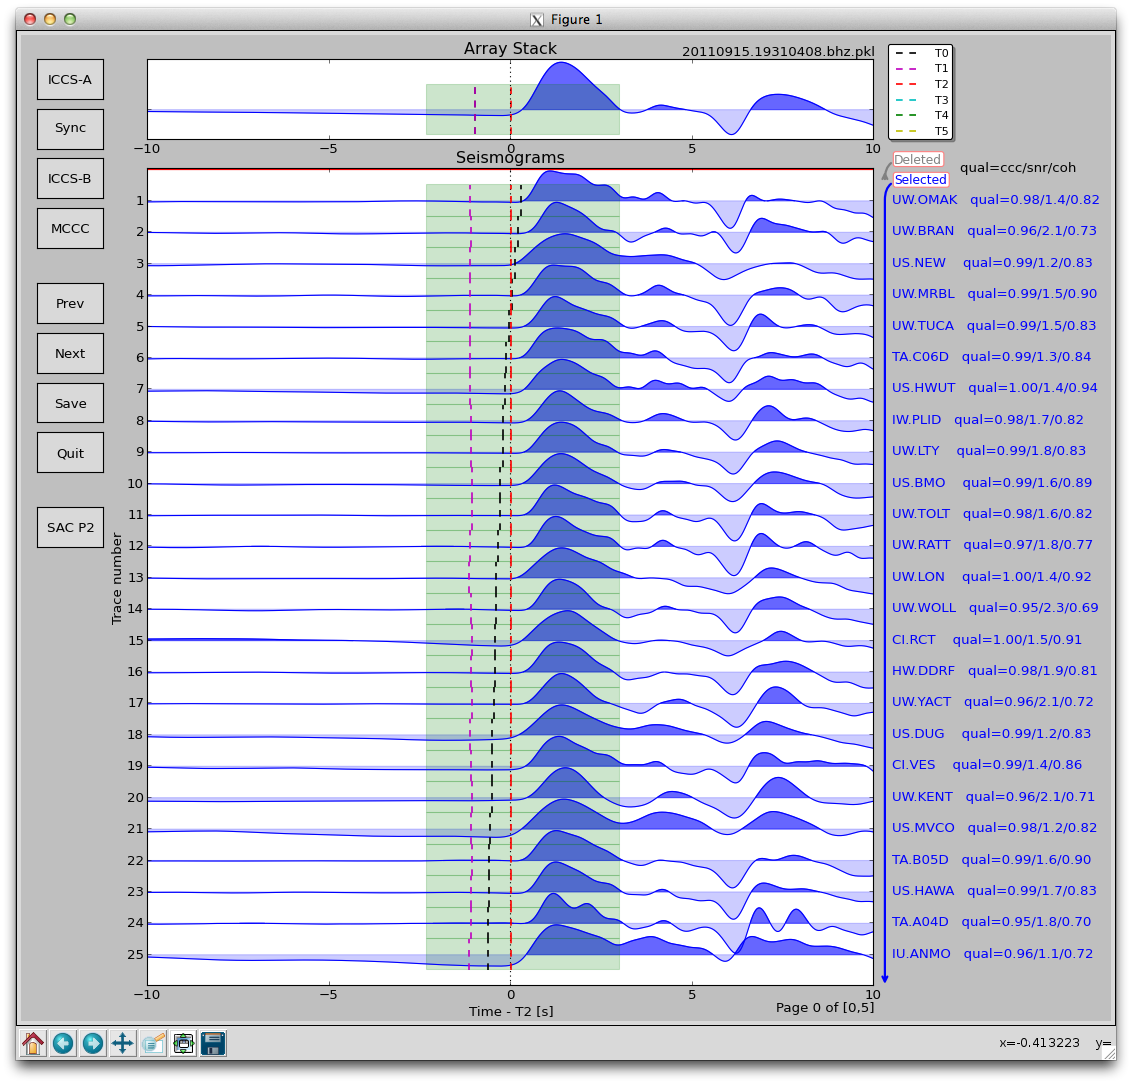
\includegraphics[width = 0.494 \textwidth]{figs/snapshots/ttpick-r2-st-increase.png}
    \caption{
    (A) Sort seismograms by time pick difference in increase order by running \texttt{"ttpick.py 20110915.19310408.bhz.pkl -x -10 10 -r2 -st"}. (B) Sort seismograms by time pick difference in decrease order by running \texttt{"ttpick.py 20110915.19310408.bhz.pkl -x -10 10 -r2 -st-"}
    }
    \label{fig:ttpick3}
\end{figure}



\begin{figure}[!h]
    \centering
    \vspace{3em}
    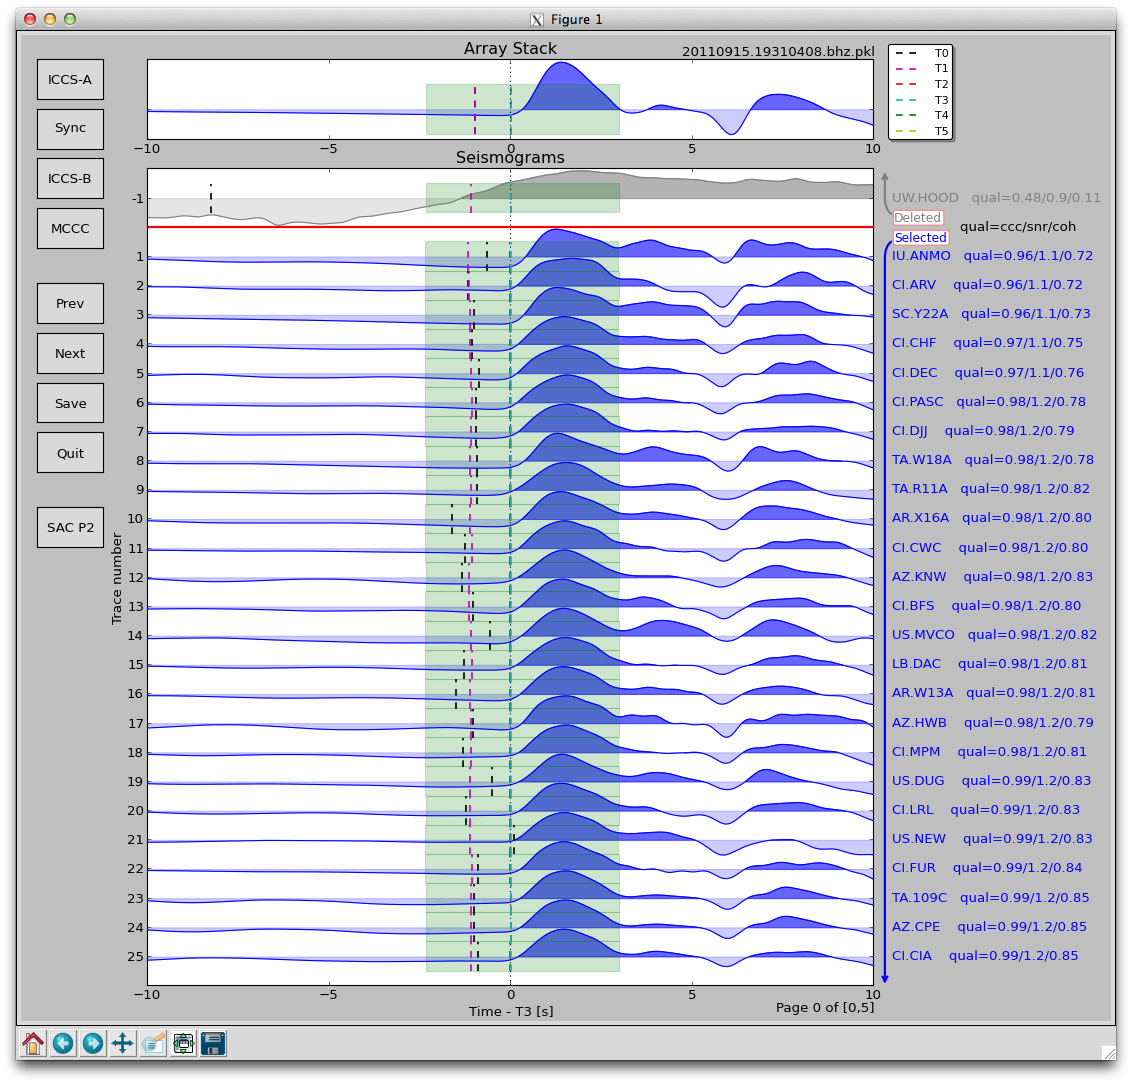
\includegraphics[width = 0.494 \textwidth]{figs/snapshots/ttpick-r3-s0.png}
    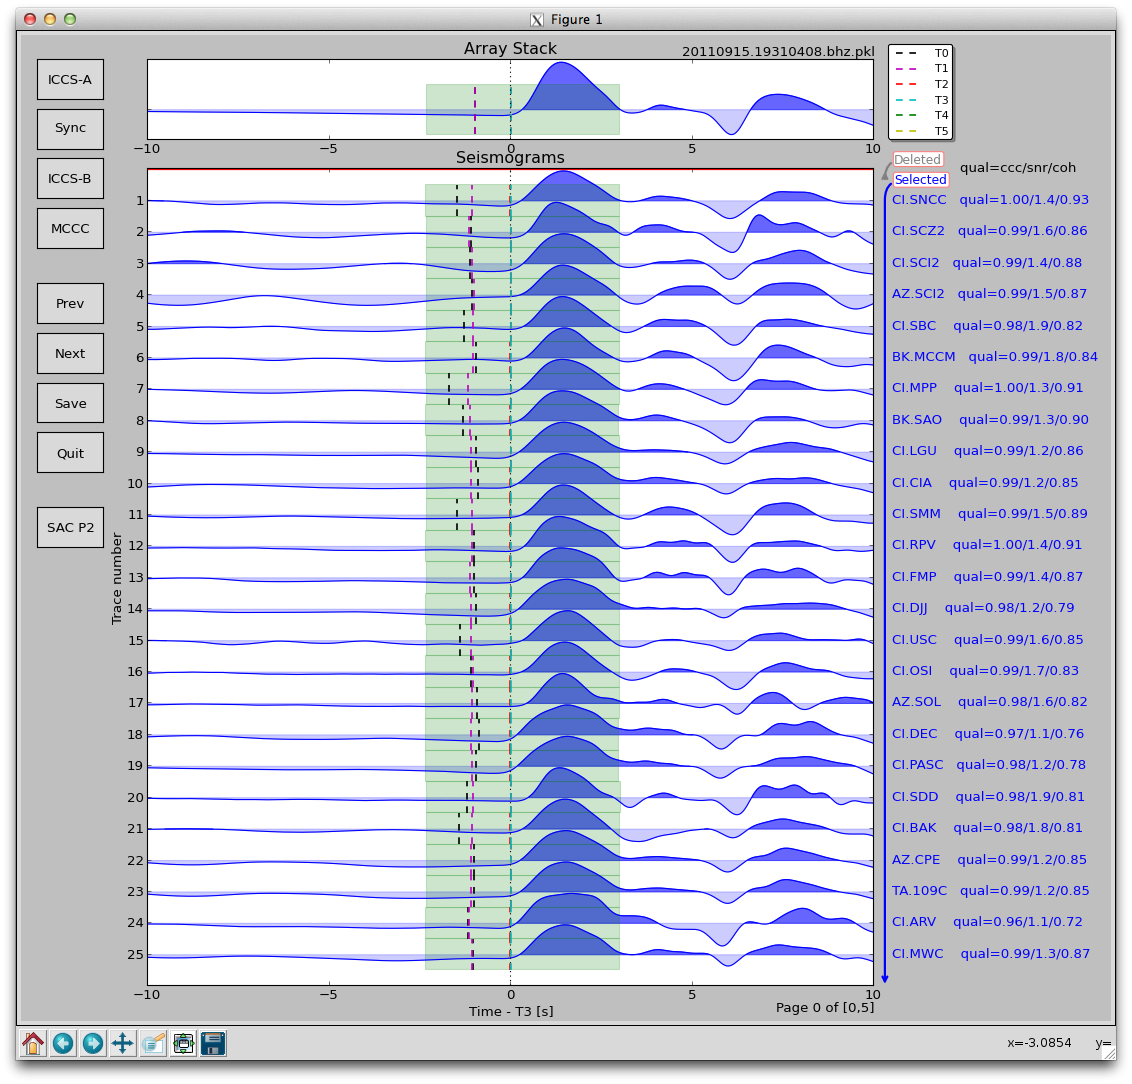
\includegraphics[width = 0.494 \textwidth]{figs/snapshots/ttpick-r3-sdist.png}
    \caption{
    (A) Run MCCC by clicking the \texttt{MCCC} Button. Relative time pick is changed from T2 to T3.
    (B) Sort seismograms by time pick difference in decrease order by running \texttt{"ttpick.py 20110915.19310408.bhz.pkl -x -10 10 -r3 -sdist"}.
    }
    \label{fig:ttpick4}
\end{figure}


%%%%%%%%%%%%%%%%%%%%%%%%%%%%%%%%%%%%%%%%%%%%%%%%%%%%%%%%
\newpage

\section{Appendix}


\appendix
\section{List of Files and Directories in the Packages}

\begin{multicols}{2}
\begin{spacing}{1}

%%%%%%%%%%%%%%%
\texttt{pysmo.sac}:
\begin{lyxcode}
setup.py

src/pysmo/sac

\hspace{2em} sacio.py

\hspace{2em} sacfunc.py

\hspace{2em} sacmeth.py

\end{lyxcode}

%%%%%%%%%%%%%%%
\texttt{pysmo.aimbat}:


\begin{lyxcode}

setup.py


src/pysmo/aimbat

\hspace{2em} algiccs.py

\hspace{2em} algmccc.py

\hspace{2em} pickphase.py

\hspace{2em} plotphase.py

\hspace{2em} plotutils.py

\hspace{2em} qualctrl.py

\hspace{2em} qualsort.py

\hspace{2em} sacpickle.py

\hspace{2em} ttconfig.py

\hspace{2em} ttdefaults.conf

\hspace{2em} xcorr.py

\hspace{2em} xcorrf.90

\hspace{2em} xcorrf90.so


scripts/

\hspace{2em} egalign1.py

\hspace{2em} egalign2.py

\hspace{2em} egplot.py

\hspace{2em} egsac.py

\hspace{2em} iccs.py

\hspace{2em} mccc.py

\hspace{2em} sac2pkl.py

\hspace{2em} sacp1.py

\hspace{2em} sacp2.py

\hspace{2em} sacpaz.py

\hspace{2em} sacpbaz.py

\hspace{2em} sacplot.py

\hspace{2em} sacppk.py

\hspace{2em} sacprs.py

\hspace{2em} ttpick.py






example/Event\_2011.09.15.19.31.04.08/

%\hspace{2em} Event\_2011.09.15.19.31.04.080

\end{lyxcode}


\end{spacing}
\end{multicols}




%
%%%%%%%%%%%%%%%
%\section{Acknowledgements}
%
%\add{We thank Dr. Gary Pavlis and the associate editor for their thoughtful reviews and suggestions.}
%We also thank Trevor Bollmann for testing the program, and Carl Ebeling, Trevor Bollmann and Emily Wolin for comments on the manuscript. 
%\add{Development of the GUI part of AIMBAT was inspired and initiated at the 2009 EarthScope USArray Data Processing and Analysis Short Course}
%(\url{http://www.iris.edu/hq/es\_course/}).
%This research is supported by NSF grant EAR-0645752 to Suzan van der Lee.
%
% 

\newpage

%%%%%%%%%%%%%%
\bibliographystyle{../../AGUManuscript/BibTeX/agufull08}
\bibliography{reference}

    


\end{document}